%\documentclass[headsepline,footsepline,footinclude=false,fontsize=11pt,paper=a4,listof=totoc,bibliography=totoc,BCOR=12mm,DIV=12]{scrbook} % two-sided
\documentclass[11pt,a4paper,listof=totoc,bibliography=totoc,openany]{scrbook} % one-sided

\usepackage{geometry}
%\usepackage[
%  top=1.25in,
%  bottom=1.25in,
%  left=1.25in,
%  right=1.25in,
%  bindingoffset=0.25in,
%  heightrounded,
%]{geometry}

\usepackage{amssymb,stmaryrd,mathrsfs,dsfont,mathtools}
\usepackage{afterpage}
\usepackage{epigraph}
\usepackage{amsthm}

\usepackage{thmtools, thm-restate}
\usepackage[dvipsnames]{xcolor} 			% einfache Verwendung von Farben in nahezu allen Farbmodellen
\usepackage[hyphens]{url}
\usepackage[Conny]{fncychap} %% Oder jarne, Bjornstrup, Glenn
\usepackage[useregional]{datetime2}
\usepackage{lipsum}
\usepackage{xspace}
\usepackage{physics}
\usepackage{enumitem}
\usepackage{awesomebox}
\usepackage{tabu}
\usepackage{tablefootnote}
\usepackage{tabularx}
\usepackage{xltabular}
% \usepackage{soul} % Nice Textdecorations, not need right now ...

\usepackage{graphics}
     \graphicspath{{fig/}}

\usepackage[style=altlist,acronym]{glossaries}
\usepackage{pgf}
\usepackage{tikz}
\usepackage{lib/tikzit}
\usepackage{caption}
\usepackage{lastpage}

\usetikzlibrary{positioning,chains,fit,shapes,calc,er,automata}
%\tikzstyle{vertex}=[circle, draw, inner sep=0pt, minimum size=6pt]

%% DECLARING STYLING
\def\hmath$#1${\texorpdfstring{{\rmfamily\textit{#1}}}{#1}}
\ChTitleVar{\bfseries\Large\rmfamily}

\ChNameVar{\bfseries\Large\sffamily}
\definecolor{applegreen}{rgb}{0.55, 0.71, 0.0}
\definecolor{aqua}{rgb}{0.0, 1.0, 1.0}

\input xy
\xyoption{all}

\setacronymstyle{long-short-desc}
\renewcommand*{\acronymentry}[1]{%
 \acronymfont{\glsentryshort{#1} -- \glsentrylong{#1}}}

\PassOptionsToPackage{table,svgnames,dvipsnames}{xcolor}

% Define TUM corporate design colors
% Taken from http://portal.mytum.de/corporatedesign/index_print/vorlagen/index_farben
\definecolor{TUMBlue}{HTML}{0065BD}
\definecolor{TUMSecondaryBlue}{HTML}{005293}
% \definecolor{TUMLightBlue}{HTML}{005293}
\definecolor{TUMSecondaryBlue2}{HTML}{003359}
\definecolor{TUMBlack}{HTML}{000000}
\definecolor{TUMWhite}{HTML}{FFFFFF}
\definecolor{TUMDarkGray}{HTML}{333333}
\definecolor{TUMGray}{HTML}{808080}
\definecolor{TUMLightGray}{HTML}{CCCCC6}
\definecolor{TUMAccentGray}{HTML}{DAD7CB}
\definecolor{TUMAccentOrange}{HTML}{E37222}
\definecolor{TUMAccentGreen}{HTML}{A2AD00}
\definecolor{TUMAccentLightBlue}{HTML}{98C6EA}
\definecolor{TUMAccentBlue}{HTML}{64A0C8}
\definecolor{VeryLightBlue}{HTML}{E8F8FF}

\definecolor{NONE}{HTML}{F721D4}
\definecolor{NTWO}{HTML}{00B1DB}
\definecolor{NTHREE}{HTML}{8C8F0E}

\definecolor{MATHAGREEN}{HTML}{B8E986}
\definecolor{MATHARED}{HTML}{E91111}
\definecolor{MATHAYELLOW}{HTML}{E6D830}

\definecolor{FILLGREEN}{HTML}{E8FFCF}
\definecolor{FILLPURPLE}{HTML}{E8FFCF}
\definecolor{FILLDARKBLUE}{HTML}{EEE6FF}

% Used for graph classes
\definecolor{darkred}{HTML}{E80000}
\definecolor{darkgreen}{HTML}{006400} 
\definecolor{yellowgreen}{HTML}{9ACD32}
% \definecolor{gray}{HTML}{E8F8FF}


\usepackage[utf8]{inputenc}
\usepackage[T1]{fontenc}
\usepackage[sc]{mathpazo}
\usepackage[ngerman,american]{babel}

\usepackage[autostyle]{csquotes}

\usepackage[%
  backend=biber,
  url=false,
  sortcites=true,
  style=numeric,
  maxnames=4,
  minnames=3,
  maxbibnames=99,
  giveninits,
  uniquename=init]{biblatex}
\usepackage{hyperref} % hidelinks removes colored boxes around references and links
\hypersetup{
colorlinks=true,
linkcolor=darkgray,
citecolor=TUMBlue,
%TODO pdftitle={Your PDF title},
pdfsubject={Parameterized Complexity},
pdfauthor={Lukas Retschmeier},
pdfkeywords={ParameterizedComplexity, Algorithms, Kernelization}
}

\usepackage{graphicx}
\usepackage{scrhack} % necessary for listings package
\usepackage{listings}
\usepackage{lstautogobble}
\usepackage{tikz}
\usepackage{pgfplots}
\usepackage{pgfplotstable}
\usepackage{booktabs}
\usepackage[final]{microtype}
\usepackage{caption}

\bibliography{bibliography}

\setkomafont{disposition}{\normalfont\bfseries} % use serif font for headings
\linespread{1.05} % adjust line spread for mathpazo font

% Add table of contents to PDF bookmarks
\BeforeTOCHead[toc]{{\cleardoublepage\pdfbookmark[0]{\contentsname}{toc}}}

% Settings for pgfplots
\pgfplotsset{compat=newest}
\pgfplotsset{
  % For available color names, see http://www.latextemplates.com/svgnames-colors
  cycle list={TUMBlue\\TUMAccentOrange\\TUMAccentGreen\\TUMSecondaryBlue2\\TUMDarkGray\\},
}

% Settings for lstlistings
\lstset{%
  basicstyle=\ttfamily,
  columns=fullflexible,
  autogobble,
  keywordstyle=\bfseries\color{TUMBlue},
  stringstyle=\color{TUMAccentGreen}
}

% Epigraphs
\setlength\epigraphwidth{.6\textwidth}
\setlength\epigraphrule{0pt}

% TIKZIT / TIKZ STYLING
\input{styling/tikz.tikzstyles}

\DeclareCaptionType{equ}[][]
\DeclareCaptionLabelFormat{blank}{}

% Reducing Spacing in new chapter
\usepackage{etoolbox}
\makeatletter
\patchcmd{\@makechapterhead}{\vspace*{50\p@}}{\vspace*{-20\p@}}{}{}
\patchcmd{\@makeschapterhead}{\vspace*{50\p@}}{\vspace*{-20\p@}}{}{}
\patchcmd{\DOTI}{\vskip 80\p@}{\vskip 0\p@}{}{}
\patchcmd{\DOTIS}{\vskip 40\p@}{\vskip 0\p@}{}{}
\makeatother
% -------------------------------------------------------------------------------------------

% REQURES FANCYHDR, BUT I DONT LIKE IT ANYMORE
% Definition der Kopf- und Fußzeilen
%\lhead{}								% Kopf links
%\chead{}								% Kopf mitte
%\rhead{\sffamily{\leftmark}}				% Kopf rechts
%\lfoot{}								% Fuß links
%\cfoot{\sffamily{\thepage}}				% Fuß mitte
%\rfoot{\sffamily{\autor}}				% Fuß rechts
%\renewcommand{\headrulewidth}{0.4pt}	% Liniendicke Kopf
%\renewcommand{\footrulewidth}{0.4pt}	% Liniendicke Fuß
%\fancyhead{}
%\lhead{}
%\chead{}
%\rhead{\textbf{\rightmark}}
%\lfoot{Lukas Retschmeier}
%\cfoot{}
%\rfoot{\thepage/\pageref{LastPage}}
%\renewcommand{\headrulewidth}{0.4pt}
%\renewcommand{\footrulewidth}{0.4pt}

% \let\thempfootnote\thefootnote


% DEPENDS ON HYPERREF
\usepackage{nameref}
\usepackage[capitalize,nameinlink]{cleveref}

% GENERAL ABBREVIATIONS
\newcommand{\mc}{\mathcal}

% ABBREVIATIONS
\newcommand{\Dvw}   {\ensuremath{\mc{D}}\xspace}
\newcommand{\Dv}    {\ensuremath{\mc{D}_{v}}\xspace}
\newcommand{\Dw}    {\ensuremath{\mc{D}_{w}}\xspace}

\newcommand{\Nthreev}    {\ensuremath{N_3(v)}}

% SETTINGS
\newcommand*{\getUniversity}{Technical University Munich }
\newcommand*{\getFaculty}{Department of Informatics}
\newcommand*{\getTitle}{On the Parametrized Complexity of Semitotal Domination on Graph Classes}
\newcommand*{\getTitleGer}{A Survey and a Linear Kernel For Planar Graphs}
\newcommand*{\getAuthor}{Lukas Retschmeier}
\newcommand*{\getDoctype}{Master Thesis}
\newcommand*{\getSupervisor}{Prof. Dr. Debarghya Ghoshdastidar (TUM)}
\newcommand*{\getAdvisor}{Prof. Dr. Paloma T. Lima (ITU)}
\newcommand*{\getSubmissionDate}{\today}
\newcommand*{\getSubmissionLocation}{København}

% TIKZ
\newcommand{\vertex}{\node[vertex]}

% COLORSKEME
\newcommand{\red}[1]{\textcolor{red}{#1}}
\newcommand{\blue}[1]{\textcolor{blue}{#1}}
\newcommand{\green}[1]{\textcolor{mygreen}{#1}}
\newcommand{\brown}[1]{\textcolor{brown}{#1}}

% THEOREM ENVIRONMENTS
\newtheorem{fact}{\protect\color{TUMSecondaryBlue} Fact}
\newtheorem{rgl}  {\protect\color{TUMSecondaryBlue} Rule} 	
\newtheorem{theorem}{\protect\color{TUMSecondaryBlue} Theorem}

\newtheorem{definition}{\protect\color{TUMSecondaryBlue} Definition}
\newtheorem{corollary}{\protect\color{TUMSecondaryBlue} Corollary}
\newtheorem{lemma}[theorem]{\protect\color{TUMSecondaryBlue} Lemma}

\newcounter{casenum}
\newenvironment{caseof}{\setcounter{casenum}{1}}{\vskip.5\baselineskip}
\newcommand{\case}[2]{\vskip.5\baselineskip\par\noindent {\bfseries Case \arabic{casenum}:} #1\\#2\addtocounter{casenum}{1}}
\crefname{case}{Case}{Cases}


\crefname{rgl}{Rule}{Rules}
\crefname{fact}{Fact}{Facts}
\crefname{theorem}{Theorem}{Theorems}
\crefname{definition}{Definition}{Definitions}
\crefname{corollary}{Corollary}{Corollaries}


\newenvironment{subproof}[1][\proofname]{%
  \renewcommand{\qedsymbol}{$\blacksquare$}%
  \begin{proof}[#1]%
}{%
  \end{proof}%
}

% ACRONYMS
\newacronym[description={Problem},%
    name={Semitotal Dominating Set}]{sds}{sds}{Semitotal Dominating Set}

\newcommand{\name}[1]{\textsc{#1}}
\newcommand{\dom}	{\name{Dominating Set}\xspace}
\newcommand{\tdom}{\name{Total Dominating Set}\xspace}
\newcommand{\sdom}{\name{Semitotal Dominating Set}\xspace}
\newcommand{\cdom}{\name{Connected Dominating Set}\xspace}
\newcommand{\rbdom}{\name{Red-Blue Dominating Set}\xspace}
\newcommand{\efdom}{\name{Efficient Dominating Set}\xspace}
\newcommand{\eddom}{\name{Edge Dominating Set}\xspace}
\newcommand{\G}		{\ensuremath{G=(V,E)}\xspace}
\newcommand{\GB}	{\ensuremath{G'=(V',E')}\xspace}
\newcommand{\R}		{\ensuremath{R(v,w)}\xspace}
\newcommand{\N}[1]	{\ensuremath{N_{#1}(v,w)}\xspace}
\newcommand{\DR}	{\ensuremath{\mc{R}}\xspace}
\newcommand{\vw}	{\ensuremath{\{ v,w\}}\xspace}
\newcommand{\sr}	{simple region}

\newcommand{\bg}	{bipartite graphs}
\newcommand{\cg}	{chordal graphs}
\newcommand{\cbg}	{chordal bipartite graphs}
\newcommand{\rpg}	{\ensuremath{r}-partite graphs}
\newcommand{\sg}	{split graphs}

\newcommand{\wtwo}	{\ensuremath{w[2]}}
\newcommand{\wone}	{\ensuremath{w[1]}}

\begin{document}

%\pagenumbering{alph}
% Set page numbering to avoid "destination with the same identifier has been already used" warning for cover page.
% (see https://en.wikibooks.org/wiki/LaTeX/Hyperlinks#Problems_with_Links_and_Pages).

\frontmatter
\afterpage{%
\newgeometry{
top=1.25in,
bottom=1.25in,
left=1.25in,
right=1.25in,
bindingoffset=0.25in,
heightrounded
}
\begin{titlepage}
  % HACK for two-sided documents: ignore binding correction for cover page.
  % Adapted from Markus Kohm's KOMA-Script titlepage=firstiscover handling.
  % See http://mirrors.ctan.org/macros/latex/contrib/koma-script/scrkernel-title.dtx,
  % \maketitle macro.
  %\oddsidemargin=\evensidemargin\relax
  %\textwidth=\dimexpr\paperwidth-2\evensidemargin-2in\relax
  %\hsize=\textwidth\relax
  \vspace*{\fill}
  \begin{center}
  \IfFileExists{logos/tum.pdf}{%
    
\includegraphics[height=20mm]{logos/tum.pdf}
  }{%
    \vspace*{20mm}
  }

  \vspace{5mm}
  {\huge\MakeUppercase{\getFaculty{}}}\\

  \vspace{5mm}
  {\large\MakeUppercase{\getUniversity{}}}\\

  \vspace{20mm}
  {\Large \getDoctype{}}

  \vspace{15mm}
  {\huge\bfseries \getTitle{}}

  \vspace{15mm}
  {\LARGE \getAuthor{}}


  \IfFileExists{logos/faculty.png}{%
    \vfill{}
    
\includegraphics[height=20mm]{logos/faculty.png}
  }{}
\end{center}
\end{titlepage}
\clearpage
\restoregeometry}

\afterpage{%
\newgeometry{
top=1.25in,
bottom=1.25in,
left=1.25in,
right=1.25in,
bindingoffset=0.25in,
heightrounded
}
% material for this page
\begin{titlepage}
  \centering
  \IfFileExists{logos/tum.pdf}{%
    
\includegraphics[height=20mm]{logos/tum.pdf}
  }{%
    \vspace*{20mm}
  }

  \vspace{5mm}
  {\huge\MakeUppercase{\getFaculty{}}}\\

  \vspace{5mm}
  {\large\MakeUppercase{\getUniversity{}}}\\

  \vspace{20mm}
  {\Large \getDoctype{}}

  \vspace{15mm}
  {\huge\bfseries \getTitle{}}

  \vspace{10mm}
  {\huge\bfseries \foreignlanguage{ngerman}{\getTitleGer{}}}

  \vspace{15mm}
  \begin{tabular}{l l}
    Author:          & \getAuthor{} \\
    Supervisor:      & \getSupervisor{} \\
    Advisor:         & \getAdvisor{} \\
    Submission Date: & \getSubmissionDate{} \\
  \end{tabular}

  \IfFileExists{logos/faculty.png}{%
    \vfill{}
    
\includegraphics[height=20mm]{logos/faculty.png}
  }{}
\end{titlepage}

\clearpage
\restoregeometry}

\afterpage{%
\newgeometry{
top=1.25in,
bottom=1.25in,
left=1.25in,
right=1.25in,
bindingoffset=0.25in,
heightrounded
}
\vspace*{0.73\textheight}
\noindent
I confirm that this \MakeLowercase{\getDoctype{}} is my own work and I have documented all sources and material used.

\vspace{15mm}
\noindent
\getSubmissionLocation{}, \getSubmissionDate{} \hspace{50mm} \getAuthor{}
\cleardoublepage{}
\clearpage
\restoregeometry}
\afterpage{%
\newgeometry{
top=1.25in,
bottom=1.25in,
left=1.25in,
right=1.25in,
bindingoffset=0.25in,
heightrounded
}
\addcontentsline{toc}{chapter}{Acknowledgments}
\thispagestyle{empty}

\vspace*{20mm}

\begin{center}
{\usekomafont{section} Acknowledgments}
\end{center}
\vspace{10mm}

Where do I even begin? 
I have so many people to thank for helping me complete this thesis, but I have to start with the one person who truly made it all possible: my supervisor, \textit{Paloma}!
Not only did you always have time for my questions and discussions, but you also showed a level of enthusiasmand passion for the problem I could not have wished more.
thank you for achieving your main mission that was to do everything to "find you a PhD programm".

I would like to express my sincere gratitude to my professor at TUM, \textit{Prof. Ghoshdastidar}, for agreeing to formally supervise my thesis. Your immediate willingness to take on this role and the uncomplicated communication was greatly appreciated!

Furthermore, I would like to thank the whole algorithms group at ITU for integrating me into the group.
From the moment I joined the group, you all made me feel welcome and included, and I am grateful for the opportunity to work in such a talented and supportive team.
Thank you to Riko for inviting me to this year's Retriet, the running sessios with Martin and Christian
% Nutan, Radu,

Special thanks goes out to Jan Arne at UiB for introducing me into the fascinating world of parameterized Complexity and engaging me to further dig into this area! 

% Atos
My employer Atos for providing me with the necessary flexibility of working hours 

Lastly, I would like to thank \textit{chatGPT Dec 15} for writing this acknowledgments section.
What a time to be alive!


\cleardoublepage{}

\clearpage
\restoregeometry}
\tableofcontents
\chapter{Abstract}
\textit{Abstract all the way}

\mainmatter~
    \chapter{Introduction}\label{ch:introduction}

\vspace*{-50pt}

\begin{figure}[ht]
        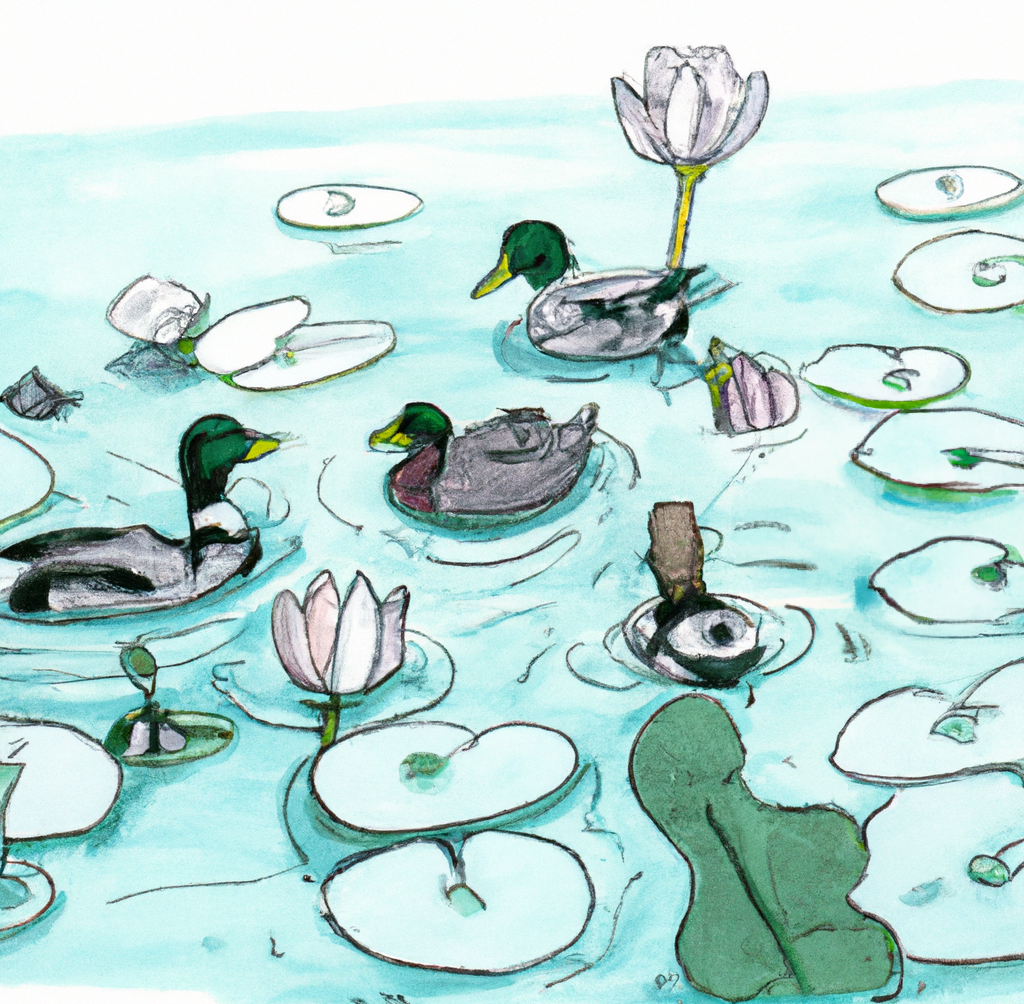
\includegraphics[width=0.35\textwidth, right]{img/dalle-ducks.png}
        \captionsetup{textformat=empty,labelformat=blank}
        \caption{Generated with Dall-E. \url{https://labs.openai.com/}. ``A duck dominating sitting on a searose''}
\end{figure}

\epigraph{\itshape Todo select another quote}{Lewis Caroll, \textit{XXXX}}

\begin{wrapfigure}{R}{0.35\textwidth}
\end{wrapfigure}

Parametrized Complexity emerging branch. Books about that

Semitotal domination was introduced by 
% TODO: Idea for a nice introduction 

Quack! Quack! Idea:  Lake with stones, and a family of ducks of fixed size want to occupy the lake so that no other clan tries to take it over.
Rules: 
* A duck can quack freeing up neighboring stones.
* Ducks don't like to be alone and want to quack together. So for every duck their must be another duck that is not further than two stones away.
Q: Can our ducklings occupy the whole lake while not feeling lonely?


TODO A demo instance next to each other 

\section{Content of the thesis}

In this thesis, we continue the systematic analysis of the \sdom problem by focusing on the parametrized complexity of the problem. 

Although the problem already had a lot of attention regarding classical complexity (CITE), only a few results are currently known for the parametrized variant. 

As far as we have seen, even the w-hardness of the general case has not been explicitly been proven in the literature. 

In this thesis, we continue the journey toward a systematic analysis by stating some hardness results for specific graph classes for the problem.

\paragraph{Our contributions}
% TODO Better: 

Our main contributions consist of first showing the $w[2]$-hardness of \sdom for XXXX graphs.

\noindent As the \dom problem and the \tdom problem both admit a linear kernel for planar graphs, it is interesting to analyze whether these results also holds for the \sdom problem which lays in between these two. 
%TODO by relxing the witness of these two provlemsproblems.

Having these kernels also for other variants like \eddom, \efdom, \cdom, \rbdom lent us great confidence that the result will also work for \sdom on planar graphs.

%% TODO Find more  .

Following the approach from ... which already relies on the technique given in, we give some simple data reduction rules for \sdom on planar graphs leading to a linear kernel. More precisely, we are going to prove the following central theorem of this thesis:

With some modifications, we were able to transfer the approach given by Garnero and Sau in \cite{Garnero2018} to the \sdom problem.

\begin{restatable}[]{theorem}{centraltheo}\label{thm:central}
    The \sdom problem parametrized by solution size admits a linear kernel on planar graphs. There exists a polynomial-time algorithms that given a planar graph $(G, k)$, either correctly reports that $(G, k)$ is a NO-instance or returns an equivalent instance $(G', k)$ such that $\abs{V(G')} \leq \kernelsize \cdot k$.
\end{restatable}

\dom problem and \tdom problem, both already 

\begin{figure}[!ht]
    \begin{equation*}
        \tikzfig{fig/tikz/ds-examples}
    \end{equation*}
    \caption[\textit{An exmaple  for a \dom, \sdom and \tdom, where $\gamma(G) < \gamma_{2t}(G) < \gamma_t(G)$ are strict.}]{\textit{An Example for Dominating Sets}}
    \label{figd:dsexamples}
\end{figure}


    \chapter{Terminology and Preliminaries}\label{ch:prelim}

\vspace*{-50pt}

\begin{figure}[ht]
        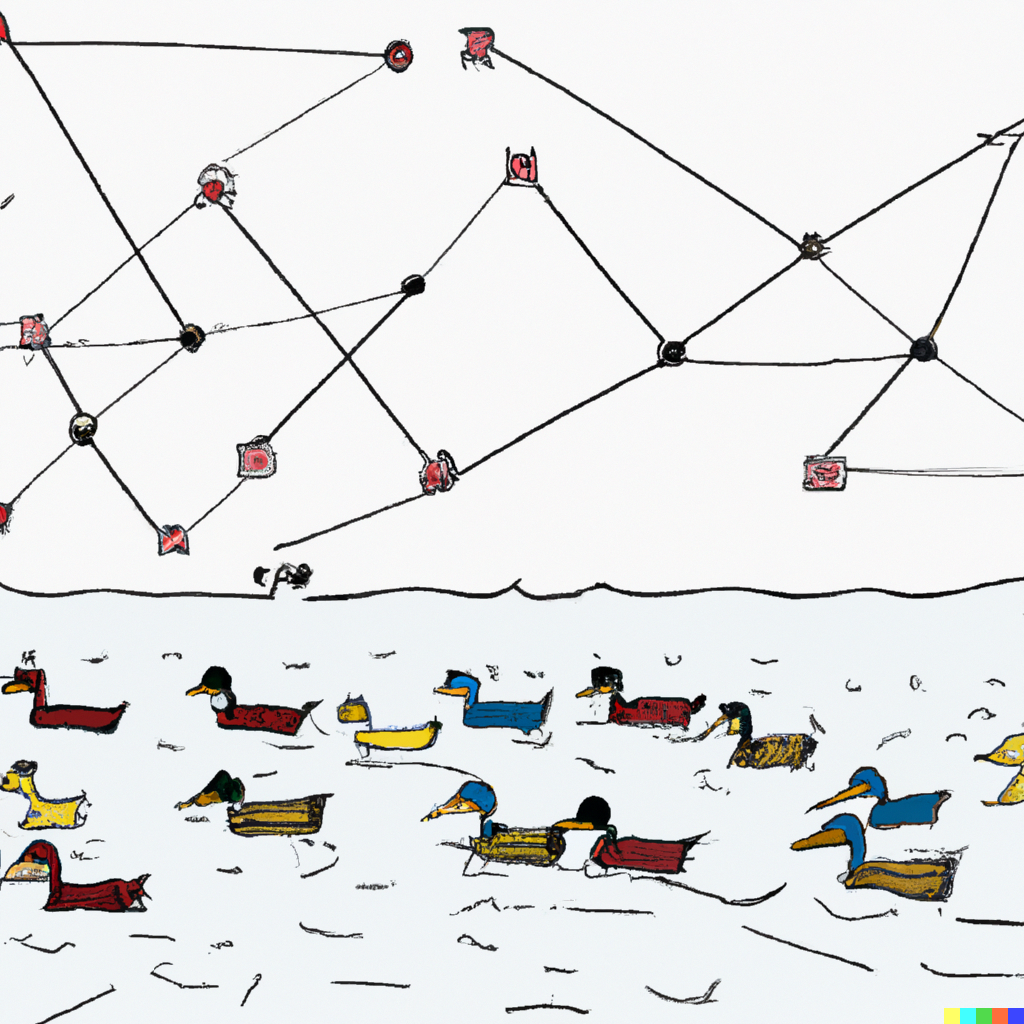
\includegraphics[width=0.35\textwidth, right]{img/gt-ducks.png}
        \captionsetup{textformat=empty,labelformat=blank}
        \caption{Generated with Dall-E. \url{https://labs.openai.com/}. ``Ducks learning graph theory while swimming on a sea sketched in color complex''}
\end{figure}

\epigraph{\itshape ``All we have to decide is what to do with the time that is given to us.''}{J. R. R. Tolkien, \textit{Gandalf} in \textit{Lord of the Rings}}


In this chapter, we will introduce the core definitions used throughout this thesis. 
Most of the definitions of graph theory are taken from \cite{Diekert2005}. 
For definitions in the area of \textit{parameterized complexity}, the book written by Cygan et al. \cite{Cygan2015} gives an excellent introduction.
For standard mathematical notation, the reader is referred to any introductory textbook into discrete mathematics (e.g. \cite{Rosen2012}).

\section{Graph Theory}

If not explicitly stated otherwise, the following definitions are taken from the book \textit{Graph Theory} written by Reinhard Diestel \cite{diestel10}.

\subsection{Basic Terminology}

\begin{definition}[Graph]
    A simple graph is a pair $G = (V, E)$ of two sets where $V$ denotes the vertices and $E \subseteq V \times V$ the edges of the graph.  A vertex $v \in V$ is incident with an edge $e \in E$ if $v \in e$. Two vertices $x, y$ are adjacent, or neighbours, if $\{x,y \} \in E$. By this definition, graph loops and multiple edges are excluded.
    
    A multigraph is a pair $(V, E)$ of disjoint sets together with a map $E \rightarrow V \cup [V]^2$ assigning to every edge either one or two vertices, its ends. Multigraphs can have loops and multiple edges.
    
    We usually denote the vertex set by $V(G)$ and its edge set by $E(G)$.


    % TODO connected 

\end{definition}

Unless stated otherwise, we usually consider only \textit{simple graphs}, but the notion of \textit{multigraphs} gets important when we later talk about the \textit{underlying multigraph} of a \dreg. 

\begin{definition}[Subgraph and Induced Subgraph]
    Let \G and $G' = (V', E')$ be two graphs. If $V' \subseteq V$ and $E' \subseteq E$ then $G'$ is a \underline{subgraph} of $G$. 
    If $G$ is a subgraph of $G'$ and $G'$ contains all the edges to $G$ with both endpoints in $V(G')$, then $G'$ is an \underline{induced subgraph} of $G$ and we write $G' = G[V(G')]$.
\end{definition}


%TODO Quote
\begin{definition}[Degrees]
    Let \G be a graph. The \textit{degree} $d_G(v)$ (shortly $d(v)$ if $G$ is clear from the context) of a vertex $v \in V$ is the number of neighbors of v. We call a vertex of degree $0$ as \underline{isolated} and one of degree $1$ as a \underline{pendant}. If all the vertices of $G$ have the same degree $k$, then $g$ is $k$-regular.
\end{definition}

% TODO Quote e.g. The open neighborhood number of a graph
\begin{definition}[Closed and Open Neighborhoods {\cite{Balakrishnan2012}}]
    Let \G be a (non-empty) graph. 
    The set of all neighbors of $v$ is the \underline{open neighborhood} of $v$ and denoted by $N(v)$; the set $N[v] = N(v) \cup \{v\}$ is the \underline{closed neighborhood} f $v$ in $G$. When G needs to be made explicit, those open and closed neighborhoods are denoted by $N_G(v)$ and $N_G[v]$. 
\end{definition}

\begin{definition}[isomorphic Graphs]
Let \G and $G' = (V', E')$ be two graphs. We call $G$ and $G'$ \underline{isomorphic}, if there exists a bijection $\phi: V \rightarrow V'$ with $\{x, y\} \in E \Leftrightarrow \phi(x)\phi(y) \in E'$ for all  $x,y \in V$. Such a map $\phi$ is called \underline{isomorphism}.

If a graph $G$ is isomorphic to another graph $h$, we denote $G \simeq H$. 
\end{definition}

\begin{definition}[Paths and Cycles]
    A path is a non-empty graph $P = (V,E)$ of the form $V = \bigcup_{i  \in [k]} \{x_i\}$ and $E = \bigcup_{i \in  [k-1]} \{x_ix_{i+1}\}$ where the $x_i$ are distinct. The vertices $x_0$ and $x_k$ are \underline{linked} by $P$ and are called the \textit{ends} of $P$. The \underline{length} of a path is its number of edges and the path on $n$ vertices is denoted by  $P_n$. We refer to a path $P$ by a natural sequence of its vertices: $P = x_0x_1...x_k$. Such a path $P$ is a path between $x_0$ and $x_k$, or a $x_0,x_k$-path.
    If $P = x_0...x_k$ is a path and $k \geq 2$, the graph with vertex set $V(P)$ and edge set $E(P) \cup \{x_kx_0\}$ is a \underline{cycle}. The cycle on $n$ vertices is denoted as $C_n$.
    The \underline{distance} $d_G(v,w)$ from a vertex $v$ to a vertex $w$ in a graph $g$ is the length of the shortest path between $v$ and $w$. If $v$ and $w$ are not linked by any path in $G$, we set $d_G(v,w) = \infty$. Again, if $G$ is clear from the context, we omit the subscripted $G$ and just write $d(v,w)$ instead.
\end{definition}

\subsection{Graph Classes}

A \textit{graph class} is a set of graphs $\mathfrak{G}$ that is closed under isomorphism that is if $G \in \mathfrak{G}$ and a $H \simeq G$ then $H \in \mathfrak{G}$ as well.

\begin{definition}[Graph Parameters]
Let \G be a graph.
An  \underline{independent set} of $G$ is a set of pairwise non-adjacent vertices. 
A \underline{clique} of $G$ is a set of pairwise adjacent vertices. 
A \underline{vertex cover} of $G$ is a subset of vertices containing at least one endpoint of every edge. 
A \underline{dominating set} is a subset $D$ of vertices such that all vertices not contained in are adjacent to some vertex in $D$.
\end{definition}

\begin{graphclass}[r-partite]
    Let $r \geq 2$ be an integer. A Graph $G = (V, E)$ is called \underline{r-partite} if $V$ admits a partition into $r$ classes such that every edge has its ends in different classes: Vertices in the same partition class must not be adjacent. 
    A \textit{$2$-partite} graph is called \underline{bipartite}. 
    
    An $r$-partite graph in which every two vertices from different partition classes are adjacent is called \underline{complete}. For the \underline{complete bipartite graph} on bipartitions $X \uplus Y$ of size $m$ and $n$, we shortly write $K_{m,n}$. 
\end{graphclass}

\begin{graphclass}[Complete]
If all vertices of a graph \G are pairwise adjacent, we say that $G$ is \underline{complete}. 
A complete graph on $n$ vertices is a $K_n$. A $K_3$ is called a \underline{triangle}.
\end{graphclass}


%\begin{definition}[{\cite[IV. Triangulated Graphs]{Berge1966}}]
%    A graph G is called \textit{chordal} (or in the older literature \textit{triangulated}) graphs if for every cycle $c = [p_1,...,p_n,p_1]$ of length $l > 3$ there is an edge of $G$ joining two non-consecutive vertices of c. Such vertices are called chords of the cycle   
%\end{definition}

\begin{graphclass}[Chordal]
For a graph \G, an edge that joins two vertices of a cycle, but is not itself an edge of the cycle is a \underline{chord} of that cycle.

Furthermore, we say $G$ is \underline{chordal} (or \textit{triangulated}) if each of its cycles of length at least four has a chord. In other words, it contains no induced cycle other than triangles.

\end{graphclass}

\begin{graphclass}[Split]
A \underline{split graph} is a graph \G whose vertices can be partitioned into a clique and an independent set.    
\end{graphclass}

%\begin{graphclass}[Bipartite {\cite[p.5]{Bondy2008}}]
%A \textit{\bg} is a Graph G whose vertex set can be partitioned into two subsets X and Y, so that each edge has one end in X and one end in Y. Such a partition (X,Y) is called a \textit{bipartition} of G.
%\end{graphclass}

%\begin{definition}[Perfect Graphs]
    
%\end{definition}

\begin{graphclass}[Planar]

A \textit{plane graph} is a pair $(V,E)$ of finite sets with the following properties:

\begin{itemize}
    \item $V \subseteq \mathbb{R}^2$ (Vertices),
    \vspace{-2mm}
    \item Every edge is an arc between two vertices, 
    \vspace{-2mm}
    \item different edges have different sets of endpoints, and
    \vspace{-2mm}
    \item The interior of an edge contains no vertex and no point of any other edge
\end{itemize}

An embedding in the plane, or \textit{planar embedding}, of an (abstract) graph $G$ is an isomorphism between $G$ and a plane graph $H$. A \textit{plane graph} can be seen as a concrete \textbf{embedding} of the planar graph into the ``plane'' $\mathbb{R}^2$.

\end{graphclass}

For an introduction into classical complexity theory. Refer to the standard textbooks aaran und cpo.
Rely an \cite[]{}
\section{Parametrized Complexity}

\paragraph{Ways to cope with NP-hard problem} Usually 

\begin{center}
    \begin{tikzpicture}
        \begin{scope}[blend mode = normal,opacity=0.75]
            \fill[red!30!white]   ( 90:1.2) circle (2);
            \fill[green!30!white] (210:1.2) circle (2);
            \fill[blue!30!white]  (330:1.2) circle (2);
        \end{scope}
        \node at ( 90:2)    {\textbf{Generality}};
        \node at ( 210:2)   {$\mathbf{\mathcal{O}(n^c)}$};
        \node at ( 330:2)   {\textbf{Exactness}};
        \node [font=\Large] {$\emptyset$};
    \end{tikzpicture}
\end{center}


\begin{definition}[Parametrized Problem{\cite[Def 1.1]{Cygan2015}}]
    A parametrized problem is a $L\subseteq\Sigma^*\times \mathbb{N}$ ($\Sigma$ finite fixed alphabet) for an instance $(x,k)\in \Sigma^*\times \mathbb{N}$, where k is called the \textit{parameter}.
\end{definition}

\begin{definition}[Instance Size]
    The \textbf{size of an instance} of an instance $(x,k)$ of a parametrized problem is $\abs{(x,k)} = \abs{x} + k$
\end{definition}
We will now clarify the basic terminology withing Parametrized Complexity. 
We are now giving a short introduction into the world of parametrized complexity. 
* General Introduction


\subsection{Fixed Parameter Tractability}

\begin{definition} [The Class FPT {\cite[Def 1.2]{Cygan2015}}]
    A parametrized problem $L\subseteq\Sigma^*\times\mathbb{N}$ is called \textit{fixed-parameter tractable} if there exists an algorithm A (called a \textit{fixed-parameter algorithm}), a computable function $f:\mathbb{N} \rightarrow \mathbb{N}$ and a constant c such that, given $(x,k) \in \Sigma^* \times \mathbb{N}$, the algorithm $\mathcal{A}$ correctly decides whether $(x,k) \in L$ in time bounded by $f(k) \cdot |(x,k)|^c$. The complexity class containing all fixed-parameter tractable problems is called \textit{FPT}
\end{definition}


\subsection{Kernelization}

\begin{definition}[kernelization Algoritm{\cite[Def 2.1]{Cygan2015}}]
A \textit{Kernelization Algorithm} or \textit{kernel} is an algorithm $\mathfrak{A}$ for a parametrized Problem Q, that given an instance $(I,k)$ of Q works in polynomial time and returns an equivalent instance $(I', k')$ of Q. Moreover, we require that $size_{\mathfrak{A}}(k) \leq g(k)$ for some computable function $g:\mathbb{N} \rightarrow \mathbb{N}$
\end{definition}

%TODO better
If we bound the size of the kernel by linear function $f(m) = \mathcal{O}(k)$, we say that the problem admits a \textbf{linear kernel}. 

%Examplary, if we reduce a graph for a graph problem in such a way that we can garuantee that our reduced graph only has a a few vertices \textbf{linear} in  $k$ left

The main idea, preprocessing algorithm, shrink size as much as possible, sound reduction rules,small output instance

\begin{definition}[Output size of a Preprocessing Procedure {\cite[p. 18]{Cygan2015}}] The output size of a preprocessing algorithms $\mathfrak{A}$ is defined as 

    \[\mathrm{size}_{\mathfrak{A}}(k) = \sup\{\abs{I'} + l': (I',k')= \mathfrak{A}(I,k), I \in \Sigma^* \} \]
\end{definition}

possibly infinite

Clearly, if there exists a kernelization algorithm for a problem $L$ and an algorithm $\mathfrak{A}$ with any runtime to decide $L$, the problem is in $FPT$ because after the kernelization pre-processing has been applied, the size of the reduced instance is a function merely in $k$ and independent of the input size $n$. In \cref{ch:linkern} we will explicitly construct a kernel for \psdom and hence showing it to be in \textit{FPT}. 

% Interstingly, als the converse?

\begin{definition}[Reduction Rules {\cite[p. 18]{Cygan2015}}]
A \textbf{reduction rule} is a function $\phi:\Sigma^* \times \mathbb{N} \rightarrow \Sigma^* \times \mathbb{N}$ that maps an instance $(x,k)$ to an equivalent instance $(x',k')$ such that $phi$ is computable in time polynomial in $\abs{x}$ and $k$
\end{definition}

\begin{definition}[Equivalent Instance {\cite[p. 18]{Cygan2015}}]
     This is a test
\end{definition}

\begin{definition}{Soundness of a rule}

\end{definition}

A \textbf{reduction rule} is a function $\Sigma* \times \mathbb{N}$ that maps an instance $(x,k)$ to an equivalent instance $(x',k')$ such that xx is computable in time polynomial in $\abs{x}$ and $k$

\subsection{Fixed Parameter Intractability: The w-Hierarchy}
\subsection{Compare to classical NP-Hardness theory}

\subsubsection{Parametrized Reductions}
\begin{definition}[Parametrized Reduction {\cite[Def 13.1]{Cygan2015}}] Let $A,B\subseteq \Sigma^*\times\mathbb{N}$ two parametrized problems. A \textit{Parametrized Reduction} from A to B is an algorithm that, given an instance $(x,k)$ of A, outputs an instance $(x', k')$ of B such that

    \begin{itemize}
        \item $(x,k)$ is a \textcolor{gray}{yes instance} of A \textbf{iff} $(x',k')$ is a \textcolor{gray}{yes instance} of B
        \item $k' \leq g(k)$ for some computable function $g$
        \item the running time is $f(k)\cdot |x|^{\mathcal{O}(1)}$ (FPT!)
    \end{itemize}
\end{definition}
    \subsubsection{The $w$-hierarchy}



\chapter{On Parameterized Semitotal Domination}\label{ch:semitotal-domination}

\vspace*{-50pt}

\begin{figure}[ht]
        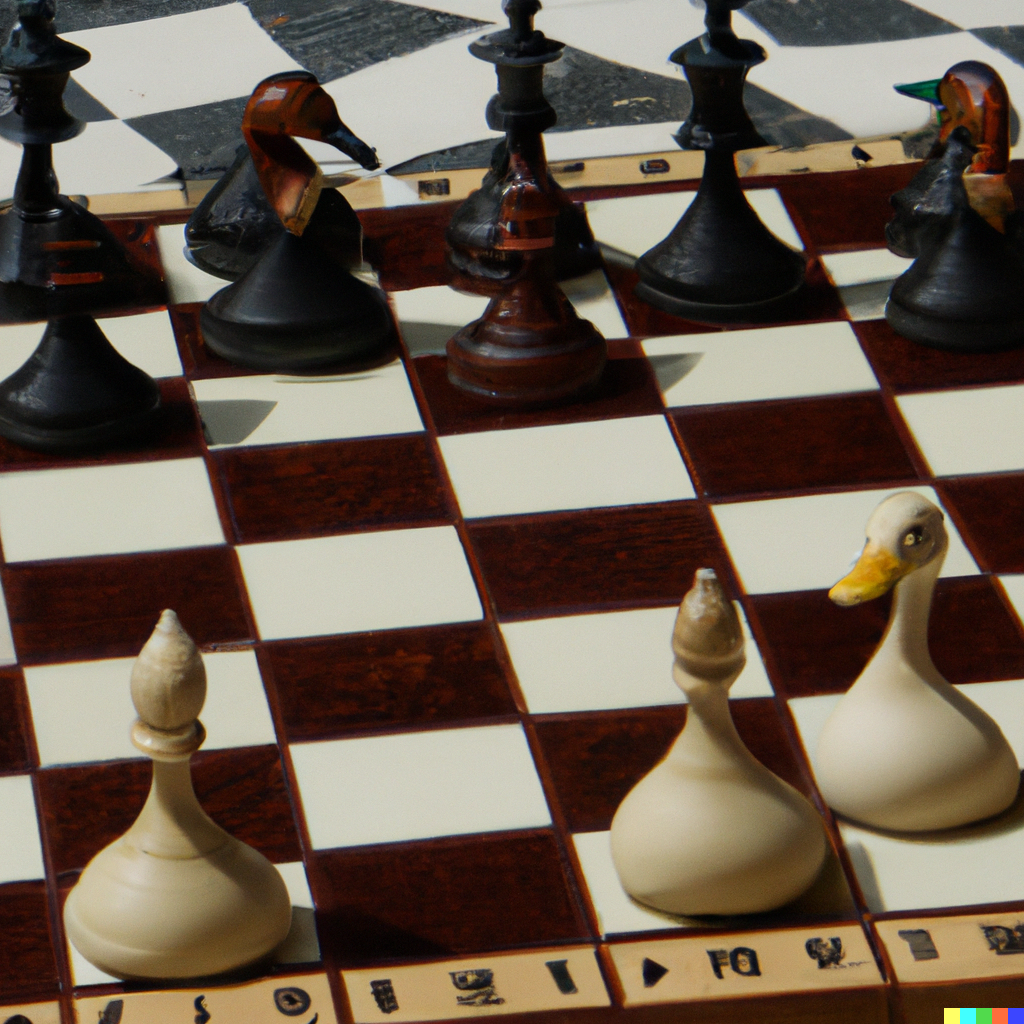
\includegraphics[width=0.35\textwidth, right]{img/chess.png}
        \captionsetup{textformat=empty,labelformat=blank}
        \caption{Generated with Dall-E. \url{https://labs.openai.com/}. ``Duck playing chess''}
\end{figure}

\epigraph{\itshape Todo select another quote}{Lewis Caroll, \textit{XXXX}}

In connection with various chessboard problems, the concept of domination can be traced back to the mid-1800s.
For example, de Jaenosch attempted in 1862 to solve the minimum number of queens required to fully cover an n x n-chessboard \cite{Jaenisch1862}. Because of the immense amount of publications related to domination, Haynes, Hedetniemi, and Slater started a comprehensive survey of the literature \cite{Haynes1998, Haynes1998b}. 
20 years later, by a series of three more books, Haynes, Henning and Hedetniemi updated the survey with the latest developments \cite{Haynes2020, Haynes2021, Haynes2022}.

After introducing the problem, we will dedicate the rest of this chapter to giving a current status about the complexity status of \dom, \sdom and \tdom on various graph classes. 
% Surprisingly, there are cases where the complexity of \dom and \tdom differes (e)
%If both \dom and \tdom are already hard for a class, we already have a strong assumption that this also holds for \sdom as well.


%Interestingly, most of them mimic each other for one specific class, but there are some exceptions, where this is not the case.

\section{The Domination Problem}

\textit{Semitotal domination} was introduced by Goddard, Henning and McPillan \cite{Goddard2014} as a relaxed form of \textit{total domination}. 

\begin{prb}[DOMINATING SET DECISION {\cite[p. 586]{Cygan2015}}]{prb:ds}
    \begin{tabularx}{0.9\textwidth}{>{\hsize=0.30\hsize}X>{\hsize=0.8\hsize}X}
        \textbf{Input:} & Graph \G and an integer $k$\\
        \textbf{Question:} & Is there a set $X \subseteq V$ of size at most $k$ such that $N[X] = V$? \\
    \end{tabularx}
\end{prb}


Goddard, Henning and McPiallan a

\begin{prb}[SEMITOTAL DOMINATING SET DECISION {\cite{Goddard2014}}]{prb:tds}
    
    \begin{tabularx}{0.8\textwidth}{>{\hsize=0.35\hsize}X>{\hsize=0.8\hsize}X}
        \textbf{Input:} & Graph \G and an integer $k$\\
        \textbf{Question:} & Is there a subset $X \subseteq V$ of size at most $k$ such that $N[X] = V$ and for all $d_1 \in X$ there exists another $d_2 \in X$ such that $d(d_1, d_2) \leq 2$?\\
    \end{tabularx}
        
\end{prb}

\begin{prb}[TOTAL DOMINATING SET DECISION {\cite[p. 596]{Cygan2015}}]{prb:sds}
    \begin{tabularx}{0.8\textwidth}{>{\hsize=0.35\hsize}X>{\hsize=0.8\hsize}X}
        \textbf{Input:} & Graph \G and an integer $k$\\
        \textbf{Question:} & Does there exists a set $X \subseteq V$ of at most $k$ vertices of G such that for every $u \in V(G)$ there exists $v \in X$ with $\{u,v\} \in E$ \\
    \end{tabularx}
        
\end{prb}

\begin{figure}
     \begin{equation*}
         \tikzfig{fig/tikz/ds-examples}
     \end{equation*}
    \caption[An example for various dominating sets]{\textit{An example for a dominating set, semitotal dominating set and a total dominating set, where $\gamma(G) < \gamma_{2t}(G) < \gamma_t(G)$ are strict. In the first case, only two vertices suffice to dominate all others. In the second one, we need a witness between $d_1$ and $d_2$ that is at most distance two. In the last case, $d_1$ and $d_2$ both need a neighbor in the total dominating set.}}
    \label{figd:dsexamples}
\end{figure}


\begin{definition}[Domination Parameters]
   The \underline{domination number} in a graph $G$ is the minimum cardinality of a dominating set of $G$, denoted as $\gamma(G)$. 
   The \underline{total domination number} is the minimum cardinality of a total dominating set (tds) of $G$, denoted by $\gamma_t(G)$.
   The \underline{semitotal domination number} is the minimum cardinality of a semitotal dominating set (sds) of $G$, denoted by $\gamma_t(G)$
\end{definition}

% Henning?


Since every total dominating set is also a semitotal dominating set and every semitotal dominating set is also a dominating set , we have the following fact first observed by Goddard and Henning \cite{Goddard2014}. 

\begin{fact}
For every graph $G$ with no isolated vertex, $\gamma(G) \leq \gamma_{t2}(G) \leq \gamma_t(G)$
\end{fact}

We can see that the semitotal domination number $\gamma_{t2}$ is squeezed between the \textit{domination} number and the \textit{total domination} number. It turns out that for some graphs, all of these inequalities can be strict. See \cref{figd:dsexamples} for an example, where $\gamma(G) < \gamma_{t2} < \gamma_t(G)$.

\subsection{Preliminaries}

* Witness
* u pendant ofrom a vertex c if $N(u) = \{w\}$
* domination 

Let $D$ be a dominating set of G and $w \in V(G) \setminus D$. For any neighbor $v \in D \cap N(w)$, we say that $d_1$ \textit{dominates} $w$ For two dominating vertices $d_1, d_2in D$. If 

Definition, dominating number

\section{Complexity Status of \sdom}\label{ch:complexity-status}

% Surprisingly, there are cases where the complexity of \dom and \tdom differes (e)
%If both \dom and \tdom are already hard for a class, we already have a strong assumption that this also holds for \sdom as well.

\section{\hmath $w[i]$-Intractibility}

Now some w[i] hard classes. 

\subsection{Warm-Up: \hmath $W[2]$-hard on General Graphs}

% TODO can we conclude anything for AT Free Graphs?
%% TODO Extend to r-partite

As any \bg with bipartition can be split further into \rpg this results also implies the \wone-hardness of \rpg


    \subsection{\hmath $W[2]$-hard on Bipartite Graphs}

\begin{definition}[Bipartite Graph, {\cite[p.5]{Bondy2008}}]
    
A \textit{\bg} is a Graph G whose vertex set can be partitioned into two subsets X and Y, so that each edge has one end in X and one end in Y. Such a partition (X,Y) is called a \textit{bipartition} of G.

\end{definition}

\begin{figure}[htb]
    \centering
\definecolor{myblue}{RGB}{80,80,160}
\definecolor{mygreen}{RGB}{80,160,80}

\resizebox{0.9\textwidth}{!}{
\begin{tikzpicture}[thick,
        every node/.style={draw,circle},
        fsnode/.style={fill=myblue},
        ssnode/.style={fill=mygreen},
        every fit/.style={ellipse,draw,inner sep=-2pt,text width=2.2cm},
        -,shorten >= 3pt,shorten <= 3pt
    ]
    % the vertices of U
    \begin{scope}[xshift=2cm,start chain=going below, node distance=7mm]
        \foreach \i in {1,2,...,5}
        \node[fsnode,on chain] (f\i) [label=above left: $x_\i$] {};
    \end{scope}

    \begin{scope}[start chain=going below, node distance=7mm]
        \foreach \i [count=\j] in {6,7,...,10}
        \node[ssnode,on chain] (f\i) [label=above left: $x'_{\j}$] {};
    \end{scope}

    % the vertices of V
    \begin{scope}[xshift=5cm,yshift=-0.5cm,start chain=going below, node distance=7mm]
        \foreach \i [count=\j] in {11,12,...,14}
        \node[ssnode,on chain] (f\i) [label=above right: $y_{\j}$] {};
    \end{scope}
    
    \begin{scope}[xshift=7cm,yshift=-0.5cm,start chain=going below, node distance=7mm]
        \foreach \i [count=\j] in {15,16,...,18}
        \node[fsnode,on chain] (f\i) [label=above right: $y'_{\j}$] {};
    \end{scope}

    \node [fsnode, left=of f8, xshift=-1cm] (nx) [label=above left: $d_1$]{};
    \node [ssnode, right=of nx, xshift=11cm] (ny) [label=above right: $d_2$]{};

    \node [ssnode, left=of nx] (nxx) [label=left: $u_1$]{};
    \node [fsnode, right=of ny] (nyy) [label=right: $u_2$]{};

    % the set U
    \node [myblue,fill=aqua, opacity=0.1,fit=(f1) (f5),label=above:$X$] {};
    \node [mygreen,fill=applegreen, opacity=0.1,fit=(f11) (f14),label=above:$Y$] {};

    \node [mygreen,fill=applegreen, opacity=0.1, fit=(f6) (f10),label=above:$ $] {};
    \node [myblue,fill=aqua, opacity=0.1, fit=(f18) (f15),label=above:$ $] {};
     
    % the set V
    % \node [mygreen,fit=(s6) (s9),label=above:$V$] {};

    % the edges
    \draw (f1) -- (f11);
    \draw (f1) -- (f12);
    \draw (f1) -- (f14);
    \draw (f2) -- (f14);
    \draw (f3) -- (f13);
    \draw (f3) -- (f11);
    \draw (f5) -- (f12);
    \draw (f4) -- (f14);
    
    \foreach \i in {6,7,...,10}
    \draw (nx) -- (f\i);

    \foreach \i in {15,16,...,18}
    \draw (ny) -- (f\i);

    \draw (ny) -- (nyy);
    \draw (nx) -- (nxx);

    % The doubled edges
    \draw (f6) -- (f1);
    \draw (f7) -- (f2);
    \draw (f8) -- (f3);
    \draw (f9) -- (f4);
    \draw (f10) -- (f5);

    \draw (f11) -- (f15);
    \draw (f12) -- (f16);
    \draw (f13) -- (f17);
    \draw (f14) -- (f18);

\end{tikzpicture}
}
\caption{Constructing G' from a bipartite Graph G by duplicating the vertices and adding a dominating tail}
\end{figure}


\begin{theorem}
    Semitotal Dominating Set is $\omega[2]$ hard for bipartite Graphs
\end{theorem}

\begin{proof}
    Given a bipartite Graph $G = ( \{X \cup Y\}, E)$, we construct a bipartite Graph G' in the following way:
    \begin{enumerate}
        \item For each vertex $x_i \in X$ we add a new vertex $x_i'$  and an edge $(x_i, x_i')$ in between.
        \item For each vertex $y_j \in Y$ we add a new vertex $y_j'$ and an edge $(y_j, y_j')$ in between.
        \item We add two $P_1$, namely $(u_1, d_1)$ and $(u_2, d_2)$, and connect them with all $(d_1, x_i')$ and $(d_2, y_j')$ respectively.
    \end{enumerate}
    \paragraph*{Observation:} G' is clearly bipartite as all $y'_j$ and $x'_i$ form again an Independent Set. Setting  $X' = X \cup \{u_2\} \cup \bigcup y'_i$ and $Y' = Y \cup \{u_1\} \cup \bigcup {x'_i}$ form the partitions of bipartite G'.

    \begin{corollary} G has a Dominating Set of size k iff G has a Semitotal Dominating Set of size $k' = k + 2$
    \end{corollary} 
    $\Rightarrow$: Asume there exists a Dominating Set D in G with size k. $DS = D\cup \{d_1,d_2\}$ is a Semitotal Dominating Set in $G'$ with size $k' = k+2 $ , because $d_1$ dominates $u_1$ and all $x'_i$; $d_2$ dominates $u_2$ and all $y'_i$. Hence, it is a Semitotal Dominating Set, because $\forall v \in (D \cap X): d(v, d_1) = 2$ and $\forall v \in (D \cap Y): d(v, d_2) = 2$

    $\Leftarrow$: On the contrary, asume any Semitotal Dominating Set $SD$ in $G'$ with size $k'$. WLOG we can asume that $u_1, u_2 \notin DS$. 
    
    Our construction forces $d_1$, $d_2 \in DS$. Because all $x'_i$ are only important in dominating $x_i$ ($y'_i$ for $y_i$ resp.) as $d_1, d_2 \in DS$. If $x'_i \in DS$ we simply exchange it with $x_i$ (for $y'_i$ and $y_i$ respectively) in our DS keeping the size of the dominating set. $D = DS \setminus \{ d_1,d_2\}$ give us a Dominating Set in G with size $ k = k' - 2$

    As G' can be constructed in $\mathcal{O}(n)$ and parameter k is only blown up by a constant, this reduction is a FPT reduction. As Dominating Set is $w[2]$ hard for bipartite Graphs\footnote{Citation needed!} so is Semitotal Dominating Set.
\end{proof}

\subsection{\hmath $W[2]$-hard on Chordal Graphs}
\begin{theorem}
    Semitotal Dominating Set is $\omega[2]$ hard on Chordal Graphs
\end{theorem}

\begin{figure}[th]
    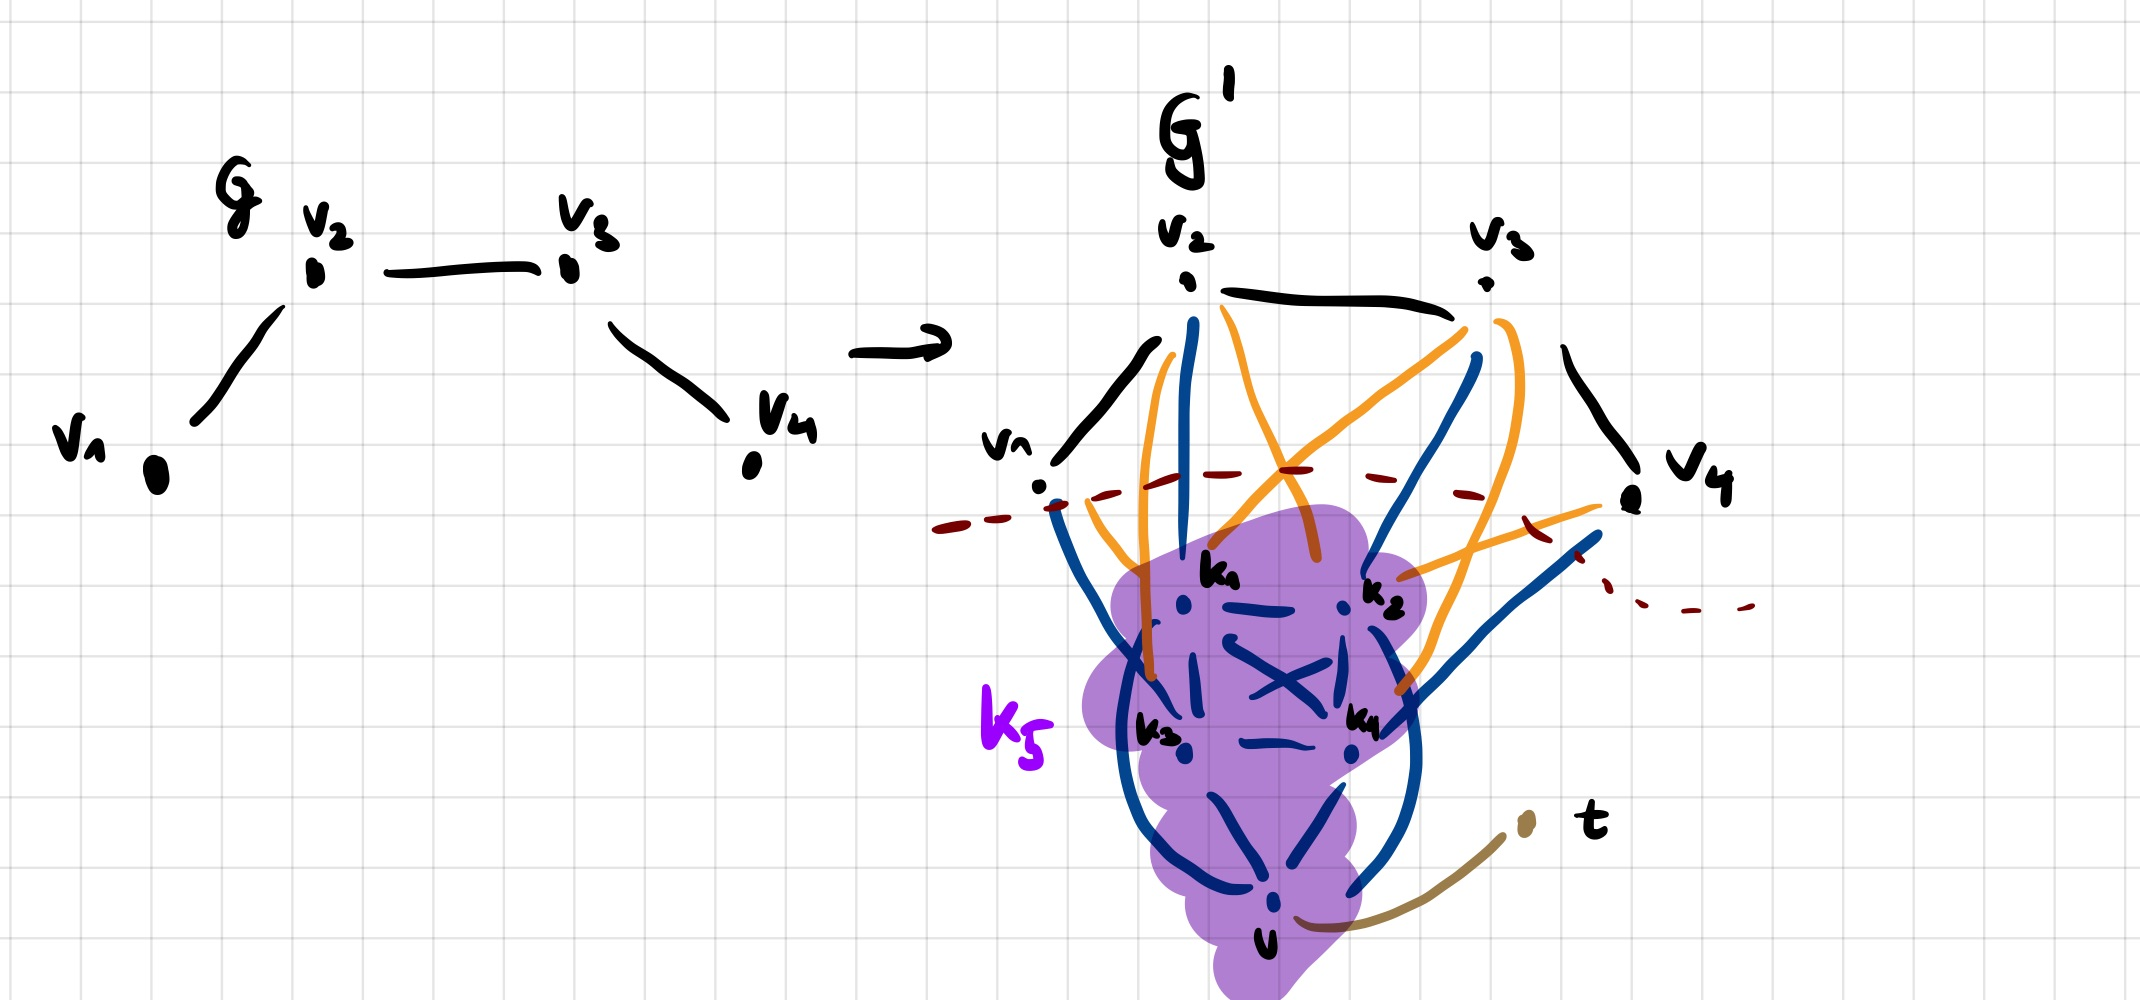
\includegraphics[scale=0.16]{pages/img/construct-chordal-reduction.jpg}
    \centering
    \caption{Constructing $G'$ by adding a $K_5$ and the vertex $t$}
    \label{fig:construct-chordal-reduction}
\end{figure}

\begin{proof}
    

    Given a chordal graph $G = (V = \{v_1,...,v_n\}, E)$, we construct a chordal graph G' as described below (See also fig \ref{fig:construct-chordal-reduction}):
    \begin{enumerate}
        \item Add a $K_{n+1}$ consisting of the vertices \{$k_1,...,k_n,u\}$ and add an edge $(v_i, k_i)$ to each vertex $v_i$ of G. One vertex $u$ in the clique will remain untouched.
        \item Add one additional vertex $t$ and connect it with $u$.
        \item For all vertices $v_i$ in G, add a new edge $(n, k_i)$ for all $n \in N(v_i)$.
    \end{enumerate}



    \begin{corollary}\label{cliqueNeighbor}
       $N(v_i) \in G$ forms a clique iff $N(v_i)$ forms a clique in $G'$
    \end{corollary}

    \begin{subproof}

\begin{figure}[th]
    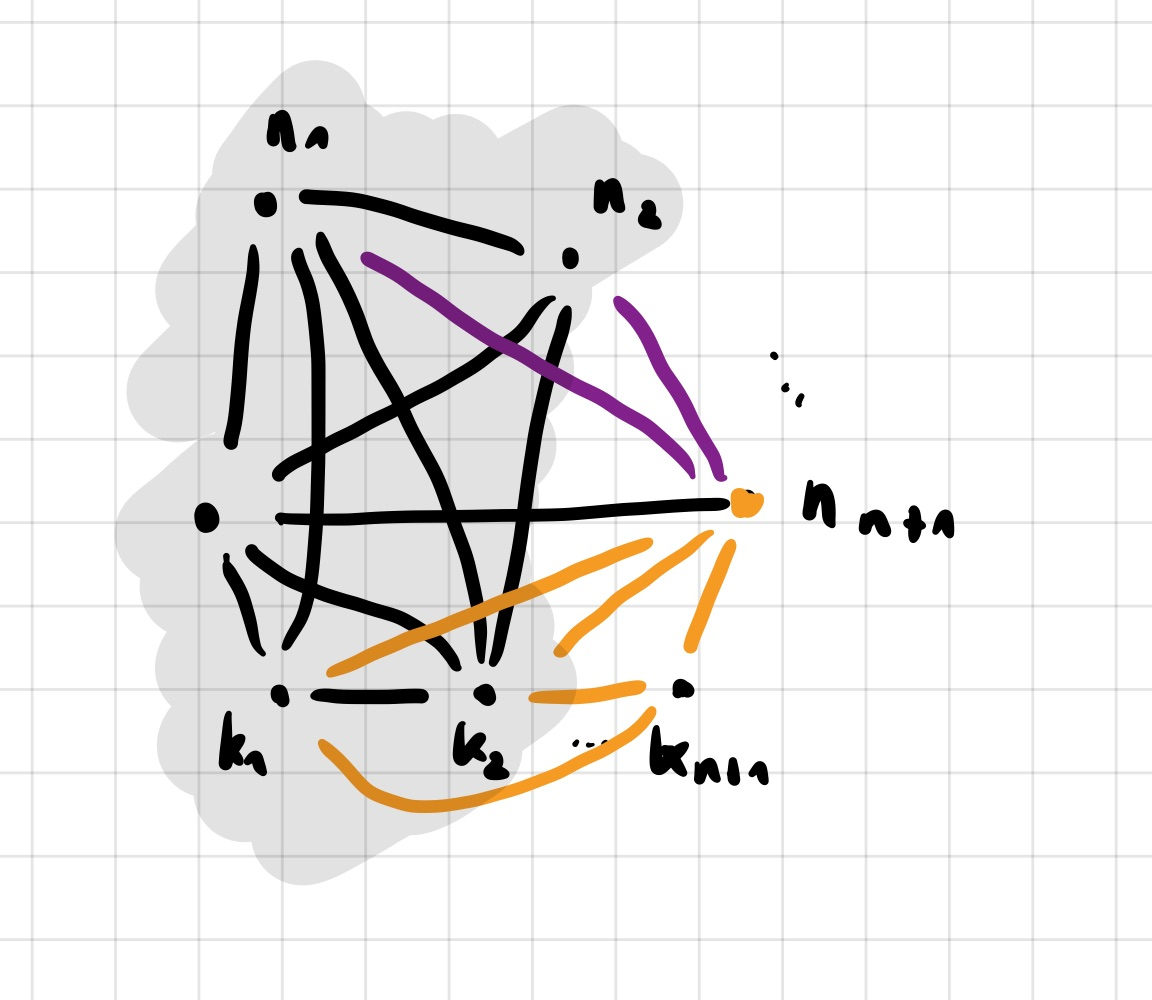
\includegraphics[scale=0.15]{pages/img/induction-step.jpg}
    \centering
    \caption{Induction Step}
    \label{fig:induction-step}
\end{figure}
        Asuming that $N(v_i)$ forms a clique in G, we show that it also forms a clique in G' by induction over the number of neighbors $z = abs(N(v_i))$ in G.

        \begin{itemize}
            \item $z = 0$: Holds trivially as we do not have a neighbor in G and in G' the connected $k_i$ forms a $P_1$, hence a clique.
            \item $z = z + 1$: 

            By IH, we already know that all neigbors $n_1,...,n_z$ form a clique together with their vertices in $k_{i}$. As $k_{z+1}, v_{z+1} \in N(v_i)$ now also in G', we show that $N(v_i)$ still forms clique in G'.

            Let $k_i$ be the vertex that was connected with $n_i$ during step 1. All we have to show is that $v_{z+1}$ and $k_{z+1}$ extend our previous clique, hence are fully connected with $N(v_i)$.
            
            $v_{z+1}$ connects to $N(v_i)$ in G by assumption. By our construction, there exists an edge to $k_1,...,k_z$, because we add an edge $(n_{z+1}, k_i)$ if there is an edge from $(n_{z+1}, n_i)$. (See fig \ref{fig:induction-step})

            $k_{z+1}$ form a complete subgraph with the other $k_i$ and is connected to all $n_i$ by construction because the edge $(n_{z+1},n_i)$ exists.  

            %Furthermore, $v_i$, $k_i$, $v_{n+1}$ and $k_{n+1}$ also form a clique, because we know that the edge $(k_i, k_{n+1})$ exists as both lay in the constructed complete induced subgraph and cross-wise edges exist from $(v_i, k_{n+1}) $ and $(v_{n+1}, k_i)$ by definition. Furthermore, $k_i$ is connected with all $N(v_{n+1})$, because $v_{n+1}$ is also a neighbor of them and hence, they must be connected to $k_i$.

            Therefore, $N(v_i)$ will also form a clique in $G'$.
        \end{itemize}

        On the other side, if $N(v_i)$ forms a clique in G', the vertices of $N(v_i)$ in G form an induced subgraph of G', hence preserving the clique.
        
    \end{subproof}
   
    \begin{corollary}
    G is Chordal iff G' is chordal.    
    \end{corollary}
    \begin{subproof}
    $\Rightarrow$: Asume $G$ chordal. Then exists a total elemination order $o = (v_1, ..., v_n)$ in G where removing $v_j$ sequentially returns cliques in $N(v_i)$.
    Define $o' = (v_1, ..., v_n, k_1, ..., k_n, u, t)$. Applying corollary \ref*{cliqueNeighbor} states that $(v_1, ... v_n)$ always gives cliques in G and according to corollary \ref*{cliqueNeighbor} also in G'. As the rest is directly part of a clique in G' by definition with an additional vertex of degree 1, o' is a total elemination order for $G'$, hence G' chordal.
    $\Leftarrow$: Holds as o' is always a total elemination order in G' and removing  the complete subgraph $K_{n+1}$ and $u$ gives a total elemination order in G.
    \end{subproof}


    \begin{corollary}
    G has a Dominating Set of size k iff $G'$ has a dominating set of size $k+1$
    \end{corollary}
    \begin{subproof}
    Asume a Dominating Set D of size k in G. $D \cup \{u\}$ is a Semitotal Dominating Set in G' of size k + 1, because $u$ dominates $t$ and for each $v \in DS: d(v, u) \leq 2$.

    Contrary, asume a Semitotal Dominating Set $SD$ in $G'$. In order to dominate $t$, $u \in SD$ must hold, hence already dominating the complete subgraph $K_{n+1}$. If a vertex $k_i \in SD$, we exchange it with $v_i$ still preserving a Dominating Set. Taking $D = SD - \{ u \}$ gives our desired Dominating Set of size k.
    \end{subproof}
    As this reduction runs in FPT time and the parameter is only bounded by a function of k, this is a FPT reduction. As Dominating Set on Chordal Graphs is $w[2]-hard$, so is SDS on Chordal Graphs.

    %TODO partial elemination order
%    \begin{corollary}
%    SDS is $w[2]$ hard on Chordal Grpahs 
 %   \end{corollary}
\end{proof}

\subsection{\hmath $W[2]$-hard on Split Graphs}

TODO Getting started with that. % Starting the actual content
    \chapter{A Linear Kernel for Planar Semitotal Domination}

\epigraph{\itshape The best way to explain it is to do it.}{Lewis Caroll, \textit{Alice in Wonderland}}

We are going to present a polynomial-time preprocessing procedure which gives a linear kernel for \psdom parametrized by solution size. Based on the technique first introduced by Alber et al. (\cite{Alber2004}) in 2004, an abundance of similar results to other domination problems emerged which gave us the believe that we can also transfer these results to \sdom. \cref{tbl:kernels} gives an overview about the status of kernels for the planar case on other domination problems. All of these results introduce reduction rules bounding the number of vertices inside so-called ``regions'' which can be obtained by a special decomposition of the graph. 

% TODO: Add running time of these algorithm there?
\begin{table}[h]
\begin{minipage}[th]{\linewidth}
\begin{tabularx}{\textwidth}{lcX}
\textbf{Problem} & \textbf{Best Known Kernel} & \textbf{Source} \\
\dom &  $67k$ & \cite{Diekert2005}\footnotemark\\
\tdom &  $410k$ & \cite{Garnero2018}\footnotemark \\
\sdom & \kernelsize & This Work \\
& & \\
\eddom & $14k$  & \cite[p. 375 - 386, Thereom 2]{Arge2007} \\
\efdom &  $84k$ & \cite[p. 375 - 386, Theorem 4]{Arge2007} \\
\rbdom &  $43k$ & \cite{Garnero2017a} \\
\cdom & $130k$  & \cite{Luo2013} \\
\dirdom &  ?  & \cite{Alber2006}  \\
\end{tabularx}
\footnotetext{There is also a masters thesis claiming a bound of 43k \cite{Halseth2016}, but a conference or journal version was not found.}
\end{minipage}
\footnotetext{Improved their own results from first $694$ \cite{Garnero2014}}
\caption{An overview about existing kernels for planar dominating set variants}
\label{tbl:kernels}
\end{table}

In the following years, this approach bore fruits in other planar problems as well like 
\name{Connected Vertex Cover}\xspace ($11/3k$ in \cite{Kowalik2013}),
\name{Maximum Triangle Packing}\xspace ($624k$ in \cite{Wang2011})
\name{Induced Matching}\xspace ($40k$ in \cite{Kanj2011})
\name{Full-Degree Spanning Tree}\xspace (TODO in \cite{Guo2006})
\name{Feedback Vertex Set}\xspace ($13k$ in \cite{Bonamy2016}) and 
\name{Cycle Packing}\xspace (\cite{Garnero2019})

In the upcoming years, many results could generalize the approach to larger graph classes. Fomin and Thilikos started this journey by directly proofing in the same year that the initial reduction rules given by Alber et al. \cite{Alber2004} can also be used to obtain a linear kernel on graphs with bounded genus g (\cite{Fomin2004}).  Alon and Gutner advanced in 2008 with showing that the problem has a linear kernel on $K_{3,h}$-topological-minor-free graph classes and a polynomial kernel for $K_h$-topological-minor-free graph classes (\cite{Gutner2009}). In 2007 they extended this result to show that graphs of bounded degeneracy are FPT (\cite{Alon2007}). Finally, in 2012 Philip et al. showed that even $K_{i,j}$-free graph classes admit a polynomial kernel for \dom (\cite{Philip2012}). 
In an attempt to extend these ideas to other problems as well, Bodlaender et al. (\cite{Bodlaender2016}) proofed that all problems expressible in  counting monadic second-order logic who sastisfy a coverability property admit a polynomial kernel on graphs of bounded genus g.

Although these results are very interesting from a theoretical point of view, the constants for the kernels obtained by these methods are so large that they are not of practical interest. The question is how such a kernel can explicitely and efficiently be constructed. 

We are going to show that, with some slight modifications, the kernel described by Garnero and Stau (\cite{Garnero2014}) for \ptdom can also be used for \psdom giving us an explicitely constructed kernel with ``reasonable'' small constants.

\section{The Main Idea}

The main idea is to use the fact that given a plane graph \G and given a vertex set $D \subseteq V$, G can be decomposed into at most $(3 \cdot \abs{D} -6)$ so-called ``regions'' (\cref{def:region}). If D is now a given \sdom~of size $k := \abs{D}$, we know that the number of regions will depend linearly on k. If we define  \textit{reduction rules}(\cref{rgl:rone,rgl:rtwo,rgl:rthree}) that try to minimize the number of vertices in and around a region we can overally bound the size of G in $k$.

As they are now, our reduction rules do not rely on the decomposition itself, but rather consider the neighborhood of every pair of vertices in the graph.

\section{Definitions}

In this section, we are giving some key definitions that are used in our reduction rules for obtaining the linear kernel. These as inspired by those given by Garnero and Stau (\ptdom in \cite[]{Garnero2014} or \prbdom in \cite{Garnero2017a}) and already relied on those given by Alber et al. in \cite[]{Alber2004} for \pdom.

The idea is to split the neighborhood of a single vertex and a pair of vertices into three distinct subsets which intuitively gives us a level of ``confinement'' of the vertices inside the neighborhood with respect to the rest of the graph (\cite{Garnero2018}). That is, they make a statement on how closely parts of the neighborhood are connected with the rest of the graph. 

\begin{definition}
    \label{def:nv}
    Let \G be a graph and let $v \in V$. We denote by $N(v) = \{u \in V : \{u,v\} \in E \}$ the neighborhood of $v$. We split $N(v)$ into three subsets:
    \begin{align}
        N_1(v) & = \{u \in N(v) : N(u) \setminus N[v] \neq \emptyset \}              \\
        N_2(v) & = \{u \in N(v)\setminus N_1(v) : N(u) \cap N_1(v) \neq \emptyset \} \\
        N_3(v) & = N(v) \setminus (N_1(v) \cup N_2(v))
    \end{align}
    In order to inhance future readability, for $i,j \in [1,3]$, we denote $N_{i,j} (v) := N_i(v) \cup N_j(v)$.
\end{definition}

\begin{figure}[!ht]
    \label{fig:neighborhoodSingle}
    \begin{equation*}
        \tikzfig{fig/tikz/neighborhoods-single-vertex}
    \end{equation*}
    \caption[The neighbordhood of a single Vertex $v$]{\textit{The neighborhood of a single vertex v split to $N_1(v)$ (purple), $N_2(v)$ (blue), and $N_3(v)$ (green). $M_1(v)$ are those having neighbors outside $N(v)$, $N_2(v)$ are a buffer between $N_1(v)$ and $N_3(v)$, and $N_3(v)$-vertices are confined in $N(v)$}}
\end{figure}

Intuitively, these sets are classifying neighbors of $v$ by how much they can interact with the rest of the graph and how much they are locally centered around $v$:

\begin{xltabular}{\textwidth}{lX}
\textbf{$\mathbf{N_1(v)}$} & are all neighbors of $v$ which have at least one adjacent vertex that is outside of $N(v)$ and therefore connect $v$ with the rest of the graph. They could possibly belong to a \sdom. \\

\textbf{$\mathbf{N_2(v)}$} & are all neighbors of $v$ that have at least one neighbor in $N_1(v)$. These vertices do not have any function as a dominating vertex and can be seen as a \textit{buffer} bridging $N_1(v)$-vertices with those from $N_3(v) \cup \{ v \}$. Furthermore, they are useless as witnesses, because either we can replace them by $v$ (sharing the same neighborhood) or when being a witness for $v$, we replace it with one $z \in N_1(v)$.\\

$\mathbf{N_3(v)}$ & vertices are sealed off from the rest of the graph. They are useless as dominating vertices: For all $z \in N_3(v)$ it holds that  $N(z) \subseteq N(v)$ by definition and thus, we would always prefer $v$ as a dominating vertex instead of $z$. Nevertheless, they can be important as a witness for $v$ in the case that $N_1(v) \cup N_2(v) =\emptyset $. We are using this observation in \cref{rgl:rone} where we shrink $\abs{N_3(v)} \leq 1$.
\end{xltabular}

% TODO What can they dominate
% TODO This sentence? Every path to a vertex outside N(v) will take more than 2 steps. 
% TODO Grammar 

Next, we are going to extend this notation also to a pair of vertices. Using this, \cref{rgl:rtwo} will later try to reduce the neighborhood of two vertice, and similar to \cref{def:nv}, we can observe nice properties. Again, the idea is to classify how strongly the shared neighborhood $N(v) \cup N(w)$ is connected with the rest of the graph.

%TODO Where is it used?
\begin{definition}
    Let \G be a graph and $v,w \in V$. We denote by $N(v,w) := N(v) \cup N(w)$ the shared neighborhood of the pair $v,w$ and split $N(v,w)$ into three distinct subsets:
    \begin{align}
        N_1(v,w) & = \{u \in N(v,w) \mid N(u) \setminus (N(v,w)\cup \{v,w\}) \neq \emptyset \}  \\
        N_2(v,w) & = \{u \in N(v,w)\setminus N_1(v,w) \mid N(u) \cap N_1(v,w) \neq \emptyset \} \\
        N_3(v,w) & =  N(v,w) \setminus (N_1(v,w) \cup N_2(v,w))
    \end{align}
    Again, for $i,j \in [1,3]$, we denote $N_{i,j}(v,w) = N_i(v,w) \cup N_j(v,w)$.
\end{definition}

$N_1(v,w)$ contains those vertices connected with the rest of the graph, $N_2(v, w)$ are a \textit{buffer} between $N_3(v,w) \cup \{v, w\}$ and $N_(v,w)$, and $N_3(v,w)$ are those vertices isolated from the rest of the graph. 

\begin{figure}[!ht]
    \begin{equation*}
        \tikzfig{fig/tikz/neighborhoods-two-vertices}
    \end{equation*}
    \caption[$N_i(v,w)$]{\textit{The neighborhood of a pair of vertices. Furthermore, note that $z \in N_1(w)$, because there is an edge to $v$, but $z \notin N_1(v,w)$ and $z \in N_3(v,w)$}}
    \label{fig:neighborhoodDouble}
\end{figure}

Note that vertices in $N_i(v)$ do not necessarily also correspond to a vertex in $N_i(v,w)$. For example \cref{fig:neighborhoodDouble} gives an example, where $z$ belongs to $N_1(v)$, but not to $N_1(v,w)$.

%\begin{figure}[ht]
%    \begin{equation*}
%        \tikzfig{fig/tikz/neighborhoods-odd}
%    \end{equation*}
%    \caption[Counterexample]{\textit{The vertex $z$ is in $N_1(v)$, because there is an edge pointing outside of $N(v)$ to $w$. Contrary, it is not in $N_1(v,w)$, but now  belongs to $N_3(v,w)$, because we are considering the ``shared'' neighborhood}}
%    \label{fig:neighborhoodWeird}
%\end{figure}

\subsection{Reduced Graph}

Before stating the reduction rules, we want to clarify when we consider a graph to be a \textit{reduced}. 

\begin{definition}[Reduced Graph {\cite[p. 13]{Garnero2018}} and \cite{Garnero2017}]\label{def:reduced}
    A Graph G is reduced under a set of rules if either none of them can be applied to G or the application of any of them creates a graph isomorphic to G.
\end{definition}

This definition differs from the definition usually given in literature where a graph G is \textit{reduced} under a set of reduction rules, if none of them can be applied to G anymore (compare e.g. \cite{Fomin2019}). Some of our reduction rules (\cref{rgl:rone} or \cref{rgl:rtwo}) could be applied \textit{ad infinitum} creating an endless loop that does not change G any more. Our definition guarantees termination in that case. All of the given reduction rules are local and only need the neighborhood of at most two vertices and replace them partially with gadgets of constant size. Now checking whether a graph after applying the rule has been isomorphically changed can be trivially accomplished in constant time.

In our case, we say G is reduced if all of the \cref{rgl:rone,rgl:rtwo,rgl:rthree} have exhaustively been applied.

\subsection{Regions in Planar Graphs}

Alber et al. (\cite{Alber2004}) introduced a novel approach on how to look at planar graphs. In their analysis they gave an construtive algorithms on how to decompose a planar graph into local areas which they call ``regions''. Vaguely said, a region is a set of vertices that are enclosed by a boundary path.

The following definitions are based on those given by Garnero and Stau (\cite{Garnero2014}) and will lead toward a clean defintion of a \textit{region} and what we understand as a \dreg.

\begin{definition}
    Two simple paths $p_1, p_2$ in a plane graph G are \underline{confluent} if:
    
    \begin{enumerate}
        \item they are vertex-disjoint
        \item they are edge-disjoint and for every common vertex $u$, if $v_i, w_i$ are the neighbors of $u$ in $p_i$, for $i \in [1,2]$, it holds that $[v_1, w_1, v_2, w_2]$, or
        \item they are confluent after contracting common edges
    \end{enumerate}
\end{definition}

% TODO MORE TEXT HERE

\begin{definition}
    Let \G be a plane graph and let $v,w \in V$ be two distinct vertices. A \underline{ region $R(v,w)$} (also denoted as $vw$-region) is a closed subset of the plane, such that:
    \begin{enumerate}
        \item the boundary of R is formed by two confluent simple $vw$-paths with length at most 3
        \item every vertex in R belongs to $N(v,w)$, and
        \item the complement of R in the plane is connected.
    \end{enumerate}
    
    We denote by $\partial R$ the boundary of R and by $V(R)$ the set of vertices which lay (with the plane embedding) in $R$. Furthermore, we call $\abs{V(R)}$ the \textit{size of the region}.
    
    The poles of R are the vertices $v$ and $w$. The boundary paths are the two $vw$-paths that form $\partial R$
    
\end{definition}

\begin{definition}
    Two regions $R_1$ and $R_2$ are non-crossing, if:
    \begin{enumerate}
        \item $(R_1 \setminus \partial R_1) \cap R_2 = (R_2 \setminus \partial R_2) = \emptyset$, and
        \item the boundary paths of $R_1$ are pairwise confluent with the ones in $R_2$
    \end{enumerate}
\end{definition}

We now have all the definitions ready to formally a maximal \dreg on planar graphs:

\begin{definition}\label{def:region}
    Given a plane graph \G and $D\subseteq V$, a \underline{$D-region$ Decomposition} of G is a set $\mathfrak{R}$ of regions with poles in D such that: 
    \begin{enumerate}
        \item for any $vw$-region $R \in \mathfrak{R} $, it holds that $D \cap V(R) = \{v, w\}$, and
        \item all regions are pairwise non-crossing.
    \end{enumerate}
    We denote $V(\mathfrak{R}) = \bigcup\limits_{R \in \mathfrak{R}} V(R)$. 
    
    \noindent A \dreg is \underline{maximal} if there is no region $R \notin \mathfrak{R}$ such that $\mathfrak{R}' = \mathfrak{R} \cup \{R\}$ is a \dreg~with $V(\mathfrak{R}) \subsetneq V(\mathfrak{R}')$.
\end{definition}


\cref{fig:maxRegionDecompose} gives an example of how to decompose a graph into a maximal $D-region$ decomposition with a given \sdom $D$ of size 3.

\begin{figure}[!ht]
    \begin{equation*}
        \tikzfig{fig/tikz/region-example}
    \end{equation*}
    \caption[Region Decomposition]{\textit{Left: A maximal \dreg $\mathfrak{R}$, where $D = \{d_1,d_2,d_3\}$ form a \sdom. There are two regions between $d_2$ and $d_1$ (purple and pink), one region between $d_1$ and $d_3$ (green) and one region between $d_2$ and $d_3$ (purple). Observe that some neighbors of $d_1$ are not part of any $vw$-region. Our reduction rules are going to take care of of them and bound these number of vertices to obtain the kernel. Right: The corresponding underlying multigraph $G_{\mathfrak{R}}$. Every edge denotes a region between $d_i$ and $d_j$}}\label{fig:maxRegionDecompose}
\end{figure}

% TODO: Wording: "kernel" prsdfecise enough here.
We are introducing a special subset of a region, namely \textit{simple region} where every vertex is a common neighbor of $v$ and $w$. They will appear in many unexpected astonishing places and are an important tool to operate on small parts of a plane graph. The upcoming \cref{rgl:rthree} will bound the size of these \textit{simple regions}. Interestingly, in the first version of the paper about the linear kernel for \ptdom (\cite{Garnero2014}), they were not given independently, but covered by one of their reduction rules (Rule 2). As it turned out, the analysis is getting simpler if we treat them in a seperate rule (In our case: \cref{rgl:rthree}) and so did Garnero and Stau in a revised version of their paper four years later (\cite{Garnero2018}).

\begin{definition}
    A simple $vw$-region is a $vw$-region such that:
    
    \begin{enumerate}
        \item its boundary paths have length at most 2, and
        \item $V(R) \setminus \{v,w\} \subseteq N(v) \cap N(w)$.
    \end{enumerate}
\end{definition}

\cref{fig:simpleRegionExample} shows an example of a simple region containing 9 distinct vertices.

\begin{figure}[!ht]
    \begin{equation*}
        \tikzfig{fig/tikz/simple-region-example}
    \end{equation*}
   \caption[A Simple Region]{\textit{A simple region with two vertices from $N_1(v,w)$ (purple) setting the boundary, two vertices from $N_2(v,w)$ (blue) and some vertices from $N_3(v,w)$ (green) in between.}}
    \label{fig:simpleRegionExample}
\end{figure}

Later we will use properties of the underlying multigraph of a \dreg. Refer to \cref{fig:maxRegionDecompose} for an example.

\begin{minipage}{\textwidth}
\begin{definition}
    Let \G be a plane graph, let $D \subseteq V$ and let $\mathfrak{R}$ be a \dreg of G. The underlying multigraph $G_\mathfrak{R} = (V_\mathfrak{R}, E _\mathfrak{R})$ of $\mathfrak{R}$ is such that  $V_\mathfrak{R} = D$ and there is an edge $\{v,w\} \in E_\mathfrak{R}$ for each vw-region $R(v,w) \in \mathfrak{R}$
\end{definition}
\end{minipage}
%% TODO: Example for a multigraph

\section{The Big Picture}

TODO Text here

\begin{figure}[!ht]
    \begin{equation*}
    \scalebox{.9}
    {
        \tikzfig{fig/tikz/overview}
    }
    \end{equation*}
    \caption[Structure of the Proof]{\textit{The plan for obtaining a linear kernel for \psdom. TODO: Check whether R1-3 apply for gray lemmas}}\label{fig:overview}
\end{figure}



% TODO for more examples refer to.
\section{Reduction Rules}

Following the approach by \cite{Garnero2014}, we are now stating reduction rules that after exhaustive application will expose a linear kernel. 

\subsection{Reduction Rule I: Getting Rid of unneccessary  $N_3(v)$ vertices}
%TODO More text:
An exemplarly application of the rule is shown in figure \ref{fig:ruleOne}

\begin{figure}[!ht]
    \begin{equation*}
        \tikzfig{fig/tikz/ruleOne}
    \end{equation*}
    \caption{\textit{TODO}}
    \label{fig:ruleOne}
\end{figure}



\begin{rgl}\label{rgl:rone}
    Let \G be a graph and let $v \in V$. If $\abs{\Nthreev} \geq 1$:
    
    \begin{itemize}
        \item remove $\Nthreev$ from G,
        \item add a vertex $v'$ and an edge $\{v, v'\}$
    \end{itemize}
    
\end{rgl}
\begin{lemma}\label{lemma:correctnessone}
    Let \G be a a graph and let $v \in V$. If $G'$ is the graph obtained by applying \cref{rgl:rone}   on $V$, then G has SDS of size k if and only if G' has one.
\end{lemma}
\begin{proof}
    This will be the proof for this lemma X 
\end{proof}

\cautionbox{Note, that we need our definition of a reduced instance given in \ref{def:reduced}. If \cref{rgl:rthree} is being applied, it will still leave us with a vertex $z\in N_3(v)$ allowing this rule to be applied again. }

\subsection{Reduction Rule II: Shrinking the Size of a Region}

% TODO: Force connectivity, improve kerne bound

% TODO: Reformulate
Extending the approach for a linear kernel for \dom proposed by Alber et al. in \cite{Alber2004}, Garnero and Stau transferred these results in \cite{Garnero2018} to the \tdom problem. 

%TODO: Better:
Their idea was to strengthen the reduction rules in such a way that the witness properties for total domination are being preserved.

% TODO Should we discuss that?
Following their approach in one of the first versions of \cite{Garnero2014}, we stating reduction rules that. Interestingly, the reduction rules given in the latest version of this paper was not directly be transferable to \sdom, but an older version giving slightly easier reduction rules could be adjusted to our problem.

which relies on the technique first introduced by Alber et al we try to reduce the neighborhood for two given vertices $v$ and $w$

Before we give the concrete reduction rule, we will define three sets 

\begin{align}
    \Dvw & = \{ \tilde D \subseteq N_{2,3}(v,w)            \mid N_3(v,w) \subseteq \bigcup_{v \in \tilde D} N(v),\ |\tilde D| \leq 3                  \} \\
    \Dv  & = \{ \tilde D \subseteq N_{2,3}(v,w) \cup \{v\} \mid N_3(v,w) \subseteq \bigcup_{v \in \tilde D} N(v),\ |\tilde D| \leq 3,\ v \in \tilde D \} \\
    \Dw  & = \{ \tilde D \subseteq N_{2,3}(v,w) \cup \{w\} \mid N_3(v,w) \subseteq \bigcup_{v \in \tilde D} N(v),\ |\tilde D| \leq 3,\ w \in \tilde D \}
\end{align}

%TODO Explain that more in detail. + Examples.

\begin{rgl}\label{rgl:rtwo}
    Let \G be a graph and two distinct $v,w \in V$. If $\Dvw = \emptyset$ we apply the following:
    \begin{caseof}
        \case{if $\Dv =  \emptyset$ and $D_w = \emptyset$}
        
        \vspace{-5mm}
        \begin{itemize}
            \item Remove $N_{2,3}(v,w)$
            \item Add vertices $v'$ and $w'$ and two edges $\{v, v'\}$ and $\{w, w'\}$
            \item If there was a common neighbor of $v$ and $w$ in $N_{2,3}(v,w)$ add another vertex $y$ and two connecting edges  $\{v, y\}$ and $\{y, w\}$
        \end{itemize}
        \case{if $\Dv \neq  \emptyset$ and $D_w \neq \emptyset$}
        % TODO: If it can not be applied any more. Using R3 to reduce this      
        Do nothing\footnote{Originally, reduce Simple Regions [STAU]}
        
        \case{if $\Dv \neq  \emptyset$ and $D_w = \emptyset$}
        
        \vspace{-5mm}
        \begin{itemize}
            \item Remove $N_{2,3}(v) \cap N_3(v,w)$
            \item Add $\{v, v'\}$
        \end{itemize}
        
        \case{if $\Dv =  \emptyset$ and $D_w \neq \emptyset$} This case is symmetrical to \textbf{Case 3}. 
    \end{caseof}
\end{rgl}


Before proofing \cref{rgl:rtwo} we will deduce some \textit{Facts} which are implied by the definitions above.

\begin{fact}
    Let \G be a graph, let $v,w \in V$, and let $G'$ be the graph obtained by the application of \cref{rgl:rtwo} on $v,w$. If $\Dvw = \emptyset$, then G has a solution if and only if it has a solution containing at least one of the two vertices $\{v,w \}$.
\end{fact}
\begin{proof}

\end{proof}

Now we are ready to proof the correctness of \cref{rgl:rtwo}

\begin{fact}
    Let \G be a graph, let $v,w \in V$, and let $G'$ be the graph obtained by the application of \cref{rgl:rtwo} on $v, w$. If $\Dvw = \emptyset$ and $\Dv = \emptyset$ (resp. $\Dw = \emptyset$) then $G'$ has a solution if and only if it has a solution containing $v$ (resp. $w$).
\end{fact}
\begin{proof}

\end{proof}

\begin{lemma}\label{lemma:correctnesstwo}
    Let \G be a plane graph, $v, w \in V$ and \GB be the graph obtained after application of \cref{rgl:rtwo} on the pair $\{v, w\}$. Then G has SDS of size k if and only if G' has SDS of size k.
\end{lemma}
\begin{proof}
    We will proof the claim by analysing the different cases seperately.
\end{proof}

\subsection{Reduction Rule III: Shrinking Simple Regions}


\begin{rgl}\label{rgl:rthree}
    Let \G be a plane graph, $v, w \in V$ and $R$ be a simple region between $v$ and $w$. If $\abs{V(R) \setminus \{v, w\}} \geq 7$
    \begin{itemize}
        \item Remove $N_3(v,w)$
        \item Add two vertices $h_1$ and $h_2$ and four edges $\{v, h_1\}$, $\{v, h_2\}$, $\{w, h_1\}$ and $\{w, h_2\}$
    \end{itemize}
\end{rgl}
\begin{lemma}[Correctness of \cref{rgl:rthree}]\label{lemma:correctnessthree}
    Let \G be a plane graph, $v, w \in V$ and \GB be the graph obtained after application of \cref{rgl:rthree} on the pair $\{v, w\}$. Then G has SDS of size k if and only if G' has SDS of size k.
\end{lemma}

The application of \cref{rgl:rthree} gives us a bound on the number of vertices inside a \sr. 
\begin{corollary}\label{lemma:simpleregionbound}
    Let \G be a graph, $v, w\in V$ and R a \sr~ between $v$ and $w$. If \cref{rgl:rthree} has been applied, this simple region has size at most 6.
\end{corollary}
% TODO Verify that
% TODO Maybe add a figure here.
\begin{proof}
    Clearly, if $\abs{V(R) \setminus \{v, w\}} < 7$ then the rule would not have changed G and the size of the region would already be bounded by 6.
    Asuming $\abs{V(R) \setminus \{v, w\}} \geq 7$ we note that every simple region can have at most two distinct vertices from $N_1(v,w)$ and two distinct ones from $N_2(v,w)$ without breaking planarity. These vertices are not touched by the reduction. Adding the two vertices that are being added between $v$ and $w$ gives us the desired upper bound.
\end{proof}


\begin{figure}[!ht]
    \begin{equation*}
        \tikzfig{fig/tikz/rulethree}
    \end{equation*}
    \caption[Application of \cref{rgl:rthree}]{\textit{TO BE DONE}}
    \label{fig:maxntwoinside}
\end{figure}


\subsection{Computing Maximal Simple Regions between two vertices}

For the sake of completeness, we state an algorithm how a maximal \sr between two vertices $v,w \in V$ can be computed in time $\mathcal{O}(d(v) + d(w))$:

\section{Bounding the Size of the Kernel}

We are now putting all our pieces together in order to proof our main result: A linear bound on the kernel size. 
In order to do so, we distinguish between those vertices that are covered by a maximal \dreg and those that are not. 
In both cases our reduction rules bound the number of vertices to a consant size which means the kernel size does only depend on the number of regions of these decomposition. 
\cref{fig:maxRegionDecompose} states that for any solution D, we only have a linear number of regions that cover the whole graph. 
In particular, we show that given a \sdom D of size k, there exist a maximal \dreg $\mathfrak{R}$ such that:

\begin{enumerate}[topsep=0pt,itemsep=-1ex,partopsep=1ex,parsep=1ex]
    \item $\mathfrak{R}$ has only at most $3 \abs{D} - 6$ regions
    \item $V(\mathfrak{R})$ covers most vertices of V. There are at most $144 \cdot \abs{D}$ vertices outside of any region.
    \item each region of $\mathfrak{R}$ contains at most XX vertices
\end{enumerate}

Combining these three parts will give us a linear kernel.

\subsection{Bounding the Size of a Region}

We start are more fine-grained analysis of the impact of the different cases of \cref{rgl:rtwo} on a $vw$-region. The main idea is to count the number of simple regions in the $vw$-region and than use the bound on the size of a simple region after \cref{rgl:rthree} was applied exhaustively and which was obtained in \cref{lemma:simpleregionbound}.   

We start by giving 

%TODO Correct Citation
\begin{lemma}\label{lemma:nonecover}
    Given a plane Graph \G and a $vw$-region R $\abs{N_1(v,w) \cap V(R)} \leq 4$ and these vertices lay exactly on the boundary $\partial R$ of $R$. 
\end{lemma}
\begin{proof}

\end{proof}

\begin{lemma}\cite[See Fact 5]{Garnero2018}\label{lemma:ntwocover}
    Given a reduced plane graph \G and a region $R(v,w)$, $N_2(v,w) \cap V(R)$ can be covered by at most 6 simple regions.
\end{lemma}
\begin{proof}
    Let $(v,u_1, u_2,w)$ and $(v, u_3, u_4, w)$ be the two boundary paths of $R(v,w)$. (A shorter path would only lead to a smaller bound).
    By definition of $N_2(v,w)$, vertices from $N_2(v,w) \cap V(R)$ are common neighbors of $v$ and $w$ and $u_i, i \in [4]$. By planarity, we can cover $N_2(v,w) \cap V(R)$ with at most 6 simple regions. To see this, imagine the graph where edges denote all possible simple $vw$-regions (See fig. \ref{fig:maxntwoinside}). There are at most 8 simple regions possible. but we have to remove at least two of them to maintain planarity.
    
    Furthermore, asuming the graph to be reduced, any intermediate $N_3(v,w)$ which could possible seperate multiple simple regions between $v$ and $u_i$ has been deleted by \cref{rgl:rone} already.
\end{proof}

\begin{figure}[!ht]
    \begin{equation*}
        \tikzfig{fig/tikz/maxntwo}
    \end{equation*}
    \caption[Bounding number of simple regions with $N_2(v,w)$ inside a $vw$-region R]{\textit{Bounding the maximum number of simple regions inside a region $R(v,w)$. $N_2(v,w)$ is covered by 6 green (simple) regions. A dashed edge would also be an option, but would contradict planarity. Note that the gray vertex g was reduced by \cref{rgl:rone} allowing the formation of exactly one simple region between $v$ and $u_1$}}
    \label{fig:maxntwoinside}
\end{figure}



We continue by giving a constant bound on the number of simple regions that cover all  $N_3(v,w)$ vertices in a given region.



%TODO: Can I "induced" in this case is undefined
\begin{lemma}\label{lemma:rtwosr}
    Given a plane Graph $G = (V,E)$ reduced under \cref{rgl:rtwo} and a region R(v, w), if $\Dv \neq $ (resp. $\Dw \neq \emptyset$), $N_3(v,w) \cap V(R)$ can be covered by: 
    \begin{enumerate}
        \item $11$ \sr s~if $\Dw \neq \emptyset$,
        \item $14$ \sr s~if $N_{2,3}(v) \cap N_3(v,w) = \emptyset$
    \end{enumerate}
\end{lemma}

Note, that the first case applies, when Case 2 \& 3 of \cref{rgl:rtwo} have been applied and the second one, when Case 4 of \cref{rgl:rtwo} was applied.
\begin{proof} 
    We will just give some intuition, because the proof of Garnero and Stau in \cite[Fact 6]{Garnero2014} does not use any special property exposed by the reduction rules. Figure (Add picture about figures) gives a visualization worst case scenarias to cover $N_3(v,w) \cap V(R)$ with simple regions in the relevant cases.\footnote{Note: In a newer revision of their paper \cite{Garnero2018}, Stau und Garnero removed this proof, because they changed \cref{rgl:rtwo} and a more fine-grained analysis was made possible.}
    
    
    % Altough our \cref{rgl:rtwo} is a bit different, the proof still goes through in the original way.
    
\end{proof}


\begin{lemma}[\#Vertices inside a Region after \cref{rgl:rone,rgl:rtwo,rgl:rthree}]\label{lemma:inside}
    Let \G be a plane graph reduced under \cref{rgl:rone,rgl:rtwo,rgl:rthree}. Furthermore, let $D$ be a SDS of G and let $v,w \in D$. Any $vw$-region R contains at most 139 vertices distinct from its poles.
\end{lemma}
\begin{proof} 
    By \cref{lemma:nonecover,lemma:ntwocover} and \cref{lemma:simpleregionbound} to bound the number of vertices inside a simple region, we know that $\abs{N_1(v,w) \cap V(R)} \leq 4$ and $\abs{N_2(v,w) \cap V(R)} \leq 6 \cdot 7 = 42$.
    
    It is still remaining to bound for \nthi, but gladly we have \cref{rgl:rtwo}, which took care about them! \cref{fig:nthreeinside} shows worst case amount of simple regions the indidual cases can have.
    
    % Maybe note that N_2 vertices do not cause any troubles as they are always bound to the near of N_1 vertex
    \begin{caseofz}
        %% TODO Check if that is correct and compare with latest paper
        \casez{If \cref{rgl:rtwo} has \textbf{not} been applied} As $\Dvw \neq \emptyset$, there exists a set $\tilde D = \{d_1,d_2,d_3\} \in \Dvw$ of at most three vertices dominating $N_3(v,w)$. We observe that vertices from \nthi~ are common neighbors of either v or w (by the definition of a $vw$-region) and at least one vertex from $\tilde D$. Withouth violating planarity, we can span at most 6 simple regions. Using \cref{lemma:simpleregionbound} and adding $\abs{\tilde D} = 3$, we can conclude $\nthi \leq 6 \cdot 6 + 3 = 39$.
        
        %% TODO even that: is it correct regarding N2?
        \casez{If \cref{rgl:rtwo} Case 1 has been applied}
        In that case \ntwi was entirely removed and at \nthi replaced by at most three vertices ($v', w'$ and $y$) added. Hence $\nthi \leq 3$.
        
        \casez{If \cref{rgl:rtwo} Case 2 has been applied} As we know that $\Dv \neq \emptyset$ and $\Dw \neq \emptyset$, we can apply \cref{lemma:rtwosr} and although \cref{rgl:rtwo} has not changed the G, we can cover R with at most $11$ simple regions giving as $\nthi \leq 11 \cdot 6 = 66$ vertices. 
        
        \casez{If \cref{rgl:rtwo} Case 3 (sym. 4) has been applied} We know that in this case $N_{2,3}(v) \cap N_3(v,w)$ was entirely removed and replaced by a single possible witness. Using \cref{lemma:rtwosr}, we can cover $(N_3(v,w) \setminus \{v'\} \cap V(R)$ with (at most) 14 simple regions giving us $\abs{\nthi} \leq 14 \cdot 6 + 1 = 85$.
    \end{caseofz}
    
    \begin{figure}[!ht]
        \begin{equation*}
            \tikzfig{fig/tikz/nthreeinside}
        \end{equation*}
        \caption[Bounding number of simple regions with inside a $vw$-region R]{\textit{TODO}}
        \label{fig:nthreeinside}
    \end{figure}
    
    All in all, as $V(R) = \{v, w\} \cup (N_1(v,w) \cup N_2(v,w) \cup N_3(v,w)) \cap V(R)$ we get 
    
    \[V(R) \leq 2 + 4 + 42 + \max(39, 3, 66, 85) = 139\]
\end{proof}

\subsection{Number of Vertices outside the Decomposition}
We continue to bound the number of vertices that do not lay inside any region of a maximal \dreg $\mathfrak{R}$, that is, we bound the size of $V \setminus \VR$. \cref{rgl:rone} ensures that we only have a small amount of $N_3(v)$-pendants. We then try to cover the rest with as few simple regions as possible, because, by application of \cref{rgl:rthree}, these simple regions are of constant size.

%Ref to 4.3

\begin{lemma}
    \cite{Alber2004}
    (Deprecated) Every vertex in $u \in V \setminus V(\mathfrak{R})$ is either in D or belongs to a set $N_2(v) \cup N_3(v)$.
\end{lemma}

The following lemma states that no vertices from a set $N_1(v)$ will be outside of a maximal \dreg.
\begin{lemma}\label{lemma:noneinside}
    \cite[Lemma 6]{Alber2004}
    Let \G be a plane graph and $\mathfrak{R}$ be a maximal \dreg of a DS D. If $u \in N_1(v)$ for some vertex $v \in D$ then $u \in V(\mathfrak{R})$
    
\end{lemma}
In the following, we define $\dGR(v) = \abs{\{R(v,w) \in \mathfrak{R}, w \in D\}}$ to be the number of regions in $\mathfrak{R}$ having $v$ as a pole. 

%TODO Add sum here
%TODO Correctness?
%% TODO Add thin underlying multigraph in theory part
\begin{corollary}
    Let \G be a graph and D be a set. For any maximal \dreg~$\mathfrak{R}$ on G it holds that $\sum_{v \in D} \dGR(v) = 2 \cdot \abs{\mathfrak{R}}$.
\end{corollary}
\begin{proof}\label{lemma:polesBound}
    
    The proof follows directly from the handshake lemma applied to the underlying multigraph~\GR.
    %    By the handshake lemma, we know that $2 \abs{E} = \sum_{v \in V} d(v)$ in a graph \G.
\end{proof}

\begin{proposition}[\#Vertices outside a Region]\label{lemma:outside}
    Let \G be a plane graph reduced under \cref*{rgl:rone,rgl:rtwo} and let D be a SDS of G. If G has a maximal D-region decomposition, then $\abs{V \setminus (V(\mathfrak{R}) \cup D)} \leq 144 \abs{D}$
\end{proposition}

With slight modifications, the proof given in \cite{Garnero2014} will also work in our case. Note that although assuming the graph to be entirely reduced, the following proof only relies on \cref*{rgl:rone,rgl:rthree}. The proof uses the observation that vertices from $N_2(v)$ span simple regions between those from $\{v\} \cup N_1(v)$.

\begin{proof}
    Again, we will follow the proof proposed by Alber et al. \cite[Proposition 2]{Alber2004}. 
    
    The proof does only rely on \cref{rgl:rone,rgl:rthree} and we can use the number of vertices in a simple region we have proofen in \cref{lemma:simpleregionbound}. In particular, we are going to proof that $V \setminus V(\mathfrak{R}) \leq 48 \cdot \abs{\mathfrak{R}} + 2 \cdot \abs{D}$. Directly placing in \cref{lemma:numRegions} will give as the desired bound.
    
    let $\mathfrak{R}$ be a maximal \dreg and let $v \in D$. Since D dominates all vertices from $V$, we can consider $V$ as $\bigcup_{v \in D}N(v)$ and thus, we only need to bound the sizes of $N_1(v)\setminus \VR$, $N_2(v) \setminus \VR$ and $N_3(v) \setminus \VR$ separately. In the following, let $v \in D$:
    %As we know that the sets $N_1(v,w)$, $N_2(v,w)$ and $N_3(v,w)$ are distinct by definition, we can seperately bound the vertices from $\abs{V \setminus V(\mathfrak{R})}$
    
    \noindent$\mathbf{N_3(v)}$: As we know that \cref{rgl:rone} has been exhaustively applied, we trivially see that $\abs{N_3(v)} \leq 1$ and hence, 
    
    \[\abs{\bigcup_{v \in D}N_3(v) \setminus V(\mathfrak{R})} \leq \abs{D}\]
    
    \noindent$\mathbf{N_2(v)}$: According to Garnero and Stau (\cite[Proposition 2]{Garnero2018}), we know that $N_2(v) \setminus V(\mathfrak{R})$ can be covered by at most $4 \dGR(v)$ simple regions between $v$ and some vertices from $N_1(v)$ on the boundary of a region in $\mathfrak{R}$. Figure \ref{fig:kernelSize} gives some intuition.
    
    Because G is reduced by assumption, we know by \cref{lemma:simpleregionbound} that a simple region can only have at least 6 vertices distinct from its poles and hence,
    
    \begin{equation}
        \begin{split}
            \abs{\bigcup_{v \in D} N_2(v) \setminus V(\mathfrak{R})} &\leq 6 \sum_{v \in D}4 \cdot \dGR(v) \\
            &= 24 \cdot \sum_{v \in D}\dGR(v) \\
            &\overset{\text{Cor. \ref{lemma:polesBound}}}{\leq} 48 \abs{\mathfrak{R}}
        \end{split}
    \end{equation}
    
    
    % TODO Now use the lemma in the revised version. 
    % TODO Formally Proof that
    % TODO Make a picture for that case 
    
    \noindent$\mathbf{N_1(v)}$: By \cref{lemma:noneinside}, we know that $N_1(v) \subseteq V(\mathfrak{R})$ and hence, 
    
    \[\abs{\bigcup_{v \in D}N_1(v) \setminus V(\mathfrak{R})} = 0\]
    
    \noindent Summing up these three upper bounds for each $v \in D$ we obtain the result using the equation from \cref{lemma:numRegions}:
    
    \begin{equation}
        \begin{alignedat}[b]{2}
            \abs{V \setminus V(\mathfrak{R}) \cup D)} &\leq 48 \cdot \abs{\mathfrak{R}} + \abs{D} & \zerotext[4em]{(Lemma \ref{lemma:numRegions})}\\ 
            &\leq 48 \cdot (3 \abs{D} - 6) + \abs{D} &\\
            &\leq 144 \abs{D} + \abs{D} &\\
            &= 145 \abs{D}
        \end{alignedat}
    \end{equation}
    
\end{proof}


\begin{figure}[!ht]
    \begin{equation*}
        \tikzfig{fig/tikz/kernelSize}
    \end{equation*}
    \caption[Vertices from $N_2(v)$ laying outside]{\textit{Bounding the number of $N_2(v)$-vertices around a dominating vertex $v$ given a maximal \dreg $\mathfrak{R}$. $v$ is a pole of $R_1, R_2,...R_j$ and can span simple regions with the help of $N_2(v)$-vertices to at most two $N_1(v)$-vertices per $R_i$. Each region has at most four vertices in $N_1(v,w) \subseteq N_1(v)$ on the boundary of $R_j$, but only at most two can be used for a simple region: Observe that trying to build a simple region between $v$ and $n_2$ in this example would contradict the maximality of $\mathfrak{R}$
            Furthermore, the size of these simple regions is bounded after the application of \cref{rgl:rthree}}}
    \label{fig:kernelSize}
\end{figure}
%

% TODO: CITE ALBER AND STAU

% TODO Maybe, we can make that simpler? No proof really uses the fact that the graph is reduced. Note, that they do not use the notion of a reduced instance in the proof.

% TODO: Shift before other parts, because this result is heavily used
\subsection{Bounding the Number of Regions}

Alber et al. \cite[Proposition 1]{Alber2004} gave a greedy algorithm to construct a maximal \dreg for a \dom. Building up on these results, Garnero and Stau gave decomposition procedures for both \rbdom (\cite{Garnero2017a}) and \tdom (\cite{Garnero2018}) relying on the same technique. This is the core of the linear kernelization, because it states that given a \dom D, we can decompose the graph into a \textit{linear number} of regions.

% TODO Better english? to span

The following lemma corresponds to \cite[Proposition 1 and Lemma 5]{Alber2004}. Although the authors gave different reduction rules and require a \textit{reduced} instance as an assumption for the following lemma, they do not use any specific properties exposed by these rules. 
As any \sdom is also a \dom, we can safely apply it for our problem as well. For a more detailed and formal proof, one can also refer to \cite[Proposition 1]{Garnero2018}.

\begin{lemma}\label{lemma:numRegions}
    Let G be a reduced plane graph and let D be a \sdom with $\abs{D}\geq 3$. There is a maximal D-region decomposition of G such that $\abs{R} \leq 3 \cdot \abs{D} - 6$
\end{lemma}
\begin{proof} 
    Follows directly from \cite[Proposition 1 and Lemma 5]{Alber2004}
\end{proof}


\begin{lemma}[Running Time of Reduction Procedure]\label{lemma:runtime}
    TODO Runsi in polynomial Time. 
\end{lemma}
\begin{proof} 
\end{proof}

\noindent By utilizing all the previous results, we are now finally ready to proof the \cref{thm:central}: 

\centraltheo*

\begin{proof}
    Let \G be the plane input graph and $G'=(V',E')$ be the graph obtained by the exhautive application of the \cref{rgl:rone,rgl:rtwo,rgl:rthree}. 
    As none of our rules change the size of a possible solution D' in G', we know by \cref{lemma:correctnessone}, \cref{lemma:correctnesstwo} and \cref{lemma:correctnessthree} that G' has a \sdom of size k if and only if G has a \sdom of size k.
    In \cref{lemma:runtime}, we have proofen that this preprocessing procedure runs in polynomial time.
    
    \noindent Asume that G' admits a solution $D'$. 
    
    %If  $\abs{D'} = 0$ then G' is empty, if $\abs{D'} = 1$, because D' needs to be a \sdom and a witness would be missing.
    
    By taking the size of each region proofen in \cref{lemma:outside}, the total number of regions in a maximal \dreg~(\cref{lemma:numRegions}) and the number of vertices that can lay outside of any region (\cref{lemma:outside}), we obtain the following bound:
    
    \begin{equation}
        139 \cdot (3k - 6) + 145 \cdot k + k \leq \kernelsize \cdot k
    \end{equation}

    \noindent If $\abs{V(G')} > \kernelsize \cdot k$ G is a NO-instance and we replace G' by two single disconnected vertices (trivial NO-instance). Then the kernel is of the claimed size.

\end{proof}

\backmatter~
  \microtypesetup{protrusion=false}
  \printbibliography
  % TODO: Discuss wether necessary. 
   \listoffigures{}
 \listoftables{}
  \microtypesetup{protrusion=true}
\appendix

\end{document}
